% VeriGraph: formal foundations of a content-addressed, contract-verified program
% representation for AI agents.
%
% Build (either works):
%   tectonic verigraph.tex
%   latexmk -pdf verigraph.tex        (pdfLaTeX + BibTeX)
%
% Every number in this paper comes from a command named in Section 8 or Appendix C.
\documentclass[11pt,a4paper]{article}

\usepackage{iftex}
\ifPDFTeX
  \usepackage[T1]{fontenc}
  \usepackage[utf8]{inputenc}
  \usepackage{lmodern}
\else
  \usepackage{fontspec}
\fi
\usepackage[margin=2.5cm]{geometry}
\usepackage{microtype}
\usepackage{amsmath,amssymb,amsthm,mathtools}
\usepackage{stmaryrd}
\usepackage{booktabs,tabularx,array}
\usepackage{enumitem}
\usepackage[dvipsnames]{xcolor}
\usepackage{listings}
\usepackage{tikz}
\usetikzlibrary{arrows.meta,positioning}
\usepackage[numbers,sort&compress]{natbib}
\usepackage[colorlinks=true,linkcolor=MidnightBlue,citecolor=MidnightBlue,urlcolor=MidnightBlue]{hyperref}
\usepackage[capitalise,nameinlink]{cleveref}
\hypersetup{
  pdftitle={VeriGraph: Formal Foundations of a Content-Addressed, Contract-Verified Program
    Representation for AI Agents},
  pdfauthor={Omar Zakaria Ben Mustapha},
  pdfkeywords={content-addressed code, program verification, SMT, IEEE 754, AI agents}
}

\setlist{itemsep=2pt,topsep=4pt}
\setlength{\emergencystretch}{3em}

% ---------------------------------------------------------------- theorems
\theoremstyle{plain}
\newtheorem{theorem}{Theorem}[section]
\newtheorem{lemma}[theorem]{Lemma}
\newtheorem{proposition}[theorem]{Proposition}
\newtheorem{corollary}[theorem]{Corollary}
\theoremstyle{definition}
\newtheorem{definition}[theorem]{Definition}
\newtheorem{assumption}[theorem]{Assumption}
\newtheorem{example}[theorem]{Example}
\theoremstyle{remark}
\newtheorem{remark}[theorem]{Remark}
\crefname{assumption}{Assumption}{Assumptions}
\crefname{lstlisting}{Listing}{Listings}
\Crefname{lstlisting}{Listing}{Listings}

% ---------------------------------------------------------------- notation
\newcommand{\VG}{VeriGraph}
\newcommand{\sem}[1]{\llbracket #1 \rrbracket}
\newcommand{\NaN}{\mathsf{NaN}}
\newcommand{\rn}{\mathrm{rn}}
\newcommand{\Z}{\mathbb{Z}}
\newcommand{\N}{\mathbb{N}}
\newcommand{\R}{\mathbb{R}}
\newcommand{\Fl}{\mathbb{F}}
\newcommand{\op}[1]{\mbox{\textsf{#1}}}
\newcommand{\kw}[1]{\texttt{#1}}
\newcommand{\eqC}{\equiv_{C}}
\newcommand{\unr}{\mathrm{unr}}
\newcommand{\pre}{\mathrm{pre}}
\newcommand{\enc}{\mathrm{enc}}
\newcommand{\dec}{\mathrm{dec}}
\newcommand{\cat}{\mathbin{\|}}
\newcommand{\Hop}{H_{\mathsf{op}}}
\newcommand{\hash}{h}
\newcommand{\Pre}{\mathit{Pre}}
\newcommand{\Post}{\mathit{Post}}
\newcommand{\val}{\mathit{val}}
\newcommand{\trap}{\mathord{\lightning}}
\newcommand{\Om}{\Omega}
\newcommand{\Eff}{\mathsf{Eff}}
\newcommand{\true}{\mathsf{tt}}
\newcommand{\false}{\mathsf{ff}}
\newcommand{\ctx}{\Gamma}
\newcommand{\file}[1]{\texttt{#1}}

% ---------------------------------------------------------------- listings
\lstdefinelanguage{vgsym}{
  morekeywords={module,NODE,SPEC,SIGNATURE,EFFECTS,CONTRACT,PRE,POST,INVARIANT,DECREASES,
    COST,BUDGET,LEARNABLE,BODY,RETURN,forall,in,result,true,false,signature,effects,pre,
    post,intent,export,loss},
  sensitive=true,
  morecomment=[l]{//},
  morestring=[b]",
}
\lstset{
  language=vgsym,
  basicstyle=\ttfamily\footnotesize,
  keywordstyle=\bfseries,
  commentstyle=\itshape\color{Gray},
  stringstyle=\color{BrickRed},
  columns=fullflexible,
  keepspaces=true,
  frame=lines,
  framesep=4pt,
  xleftmargin=6pt,
  xrightmargin=6pt,
  aboveskip=8pt,
  belowskip=6pt,
  captionpos=b,
  upquote=true,
  showstringspaces=false,
}

\title{\VG: Formal Foundations of a Content-Addressed,\\
  Contract-Verified Program Representation for AI Agents}
\author{Omar Zakaria Ben Mustapha\thanks{The repository is private at the time of writing and is
  scheduled to become public at milestone M1. Every measurement in this paper names the
  commit and the command that produced it (\cref{sec:status,app:repro}).}}
\date{Draft of 6 November 2026 \\[2pt] \small Prototype commit \texttt{fe499c8}}

\begin{document}
\maketitle

\begin{abstract}
\noindent
\VG{} is a programming system designed for software written, checked and repaired by AI
agents. A program is a set of nodes; each node is a typed, single-assignment dataflow graph of
combinators with a machine-checked contract, and its identity is a BLAKE3 hash of its
canonical structure and contract. Contracts are split into obligations, each discharged by
one quantifier-free SMT query, and every failure is returned as structured data with a
counterexample that a reference interpreter replays. This paper gives the formal
foundations of the design. We define a core calculus for nodes and prove that:
(i)~two bodies have the same hash if and only if their unravelings coincide up to the
commutativity of designated operations, under an explicit field-capacity condition and the
standard collision-freeness idealization, and that hash equality implies equal meaning;
(ii)~hash-consing never merges two effect operations when effect tokens are linear;
(iii)~no polynomial-time canonical form identifies exactly the semantically equivalent nodes
unless $\mathrm{P}=\mathrm{NP}$, which justifies identity by specification;
(iv)~identifying all NaN bit patterns makes every float operation of the minimal viable
product a congruence, except copySign with a NaN sign operand, and makes addition,
multiplication, minimum and maximum commutative bit for bit;
(v)~the combinator proof rules, the fresh-element rule and an exact bit-width encoding of
mathematical integers are sound, provided each obligation is checked only against facts of
operations that precede it in a topological order, a proviso we show to be necessary.
We give a complete IEEE~754 proof of the case study's soft-knee kernel and characterize
exactly the inputs on which its first draft fails; an exhaustive check of every finite
binary32 input for ten knee values ($4.28\times10^{10}$ evaluations) agrees. Finally, we report
the prototype: its core representation passes the automated checks of its first gate, which
still awaits the owner's approval, and an independent review found violations of exactly our
side conditions, among them a hash collision that we reproduce. No verifier, compiler or
benchmark exists yet, and we claim none.
\end{abstract}

\tableofcontents
\bigskip

\section{Introduction}\label{sec:intro}

AI agents now write, test and repair code in loops with little human involvement. The
artifacts they manipulate were designed for human authors: a program is a set of text files
whose identity is a path, whose meaning depends on names and declaration order, whose
diagnostics are prose, and whose compiled behaviour may depend on undefined behaviour and on
the floating-point unit of the target. Verification-aware languages such as
Dafny~\cite{leino2010dafny}, Why3~\cite{filliatre2013why3}, F*~\cite{swamy2016fstar} and
Verus~\cite{lattuada2023verus} close part of the gap: a program carries a contract that a
solver checks, and language models are becoming competent at writing such
programs~\cite{bursuc2025vericoding}. Identity, error reporting, determinism and composition
nevertheless remain organized around text written for people.

\VG{} starts from a different question: what should a program representation look like if
every design decision is judged by what it does for an agent that writes, checks and repairs
code with no human in the loop? Its answer has four parts.
\begin{enumerate}
\item A program is a set of \emph{nodes}. Each node is one function: a typed,
  single-assignment dataflow graph of combinators, with a contract (pre- and postconditions,
  loop invariants, cost bounds) and an effect set. Its identity is a BLAKE3
  hash~\cite{blake3} of its canonical structure and contract, so equal programs have equal
  names on every machine and every proof can be cached by content.
\item Agents write a textual projection, VG-Sym, in which they name things with labels; the
  toolchain computes every hash. Ports and labels are defined before use, so every prefix of
  a VG-Sym file can be checked.
\item Each contract is split into \emph{obligations}, each discharged by one quantifier-free
  SMT query in a fragment that Z3~\cite{demoura2008z3}, cvc5~\cite{barbosa2022cvc5} and
  Bitwuzla~\cite{niemetz2023bitwuzla} all accept. A failure comes back as structured data: an
  obligation identifier, a counterexample that a reference interpreter replays, and a failing
  slice of the graph.
\item Verified nodes are meant to compile, through textual LLVM IR~\cite{lattner2004llvm}, to
  x86\_64, ARM64 and WebAssembly binaries that agree bit for bit with the interpreter, with
  proven facts turned into optimization hints and an operating-system sandbox derived from the
  capabilities of the root node.
\end{enumerate}

These choices raise precise questions that an informal specification answers only loosely.
When do two programs share a hash, and when must they not? Can effectful operations be merged
by hash-consing? What does a floating-point value \emph{mean} when x86\_64, AArch64 and
WebAssembly disagree on the bits of NaN? Which proof rules make bounded loops verifiable with
quantifier-free queries, and are they sound? What does a counterexample that does not replay
tell the agent? This paper answers these questions with definitions, theorems and proofs.

\paragraph{Contributions.}
\begin{itemize}
\item A core calculus for \VG{} nodes (\cref{sec:calculus}): types with a one-NaN float
  domain, nodes as term graphs with linear effect tokens, a strict evaluation semantics with
  traps, contracts with explicitly unspecified values, and two confinement results: a node's
  effects stay within its declared set, and capabilities cannot be forged.
\item A characterization of content addressing (\cref{sec:identity}). Under an explicit
  field-capacity condition and the usual collision-freeness idealization, two bodies have the
  same hash if and only if their unravelings coincide up to commutativity
  (\cref{thm:hash-char}); equal node hashes imply equal meaning (\cref{thm:hash-meaning}); and
  hash-consing never merges two effectful operations when effect tokens are linear
  (\cref{lem:eff-never-merged}). We also prove that no polynomial-time canonical form
  identifies exactly the semantically equivalent nodes unless $\mathrm{P}=\mathrm{NP}$
  (\cref{thm:conp}), which justifies the design's identity by specification.
\item A one-NaN semantics for IEEE~754 (\cref{sec:float}). Identifying all NaN bit patterns
  makes every float operation of the minimal viable product (MVP) a congruence, except
  copySign with a NaN sign operand, which the design therefore treats as partial
  (\cref{thm:float-congruence}). Under this semantics addition, multiplication, minimum,
  maximum and the product part of a fused multiply-add are commutative bit for bit
  (\cref{thm:float-comm}), which licenses sorting their operands during canonicalization.
\item Soundness of modular verification (\cref{sec:verification}). The combinator proof
  rules, the fresh-element rule and an exact bit-width encoding of mathematical integers
  (\cref{thm:widths}) are sound (\cref{thm:soundness}), provided each obligation is checked
  only against facts of operations that precede it in a topological order. A four-operation
  program shows that this proviso is necessary (\cref{prop:ordering-needed}); the current
  specification does not state it. The counterexample-replay classification is sound too
  (\cref{thm:replay}).
\item A complete IEEE~754 proof that the case study's soft-knee kernel meets its contract,
  and an exact characterization of the inputs on which its first draft fails
  (\cref{sec:case}), cross-checked exhaustively on every finite binary32 input for ten knee
  values, $4.28\times10^{10}$ evaluations.
\item An honest account of the prototype (\cref{sec:status}): what exists, what it passes, and
  the findings of an independent review, two of which we reproduce and show to be exactly
  violations of the side conditions of our theorems.
\end{itemize}

\paragraph{Status and scope.}
\VG{} is at an early stage. Its core intermediate representation (parser, printer,
canonicalizer, hashing, binary codec and object store) is implemented in about 9,600 lines of
Rust, tests included. The type checker, interpreter, verifier, code generator, agent loop,
registry and lifter are specified but not implemented. Our theorems are about the
specification and the core calculus, not about running code; where we report a measurement,
we name the commit and the command. We make no claim about verification time, the speed of
generated code or synthesis success rates, because none of them has been measured.

\paragraph{Organization.}
\Cref{sec:overview} introduces \VG{} through its case study. \Cref{sec:calculus} defines the
core calculus. \Cref{sec:identity} studies identity and content addressing,
\cref{sec:float} floating point, and \cref{sec:verification} verification.
\Cref{sec:case} proves the case study correct. \Cref{sec:status} reports the prototype,
\cref{sec:related} discusses related work and \cref{sec:discussion} the limitations.

\section{\VG{} by example}\label{sec:overview}

The running example is the milestone the project must reach first. Its plain-language request
reads: \emph{write a verified real-time audio limiter that takes a 512-sample stereo FP32
buffer, clamps peaks smoothly using a learnable knee threshold so that no sample ever exceeds
$[-1, 1]$, computes a SHA-256 digest of the output frame, and runs in under 500 microseconds
with zero heap allocation.} \Cref{lst:softknee,lst:frame} show the reference solution,
verbatim from \file{examples/audio\_limiter.vgs}.

\subsection{Nodes, ports and contracts}

\begin{lstlisting}[float=t,caption={The soft-knee kernel, repaired version.},label=lst:softknee]
NODE @soft_knee [intent: "Soft-knee clip of one sample into [-1, 1]"] {
  SIGNATURE: (x: f32, knee: f32) -> (f32);
  EFFECTS: [];
  CONTRACT {
    PRE:  is_finite(x) && knee >= 0.5 && knee <= 0.99;
    POST: result >= -1.0 && result <= 1.0 && ((x >= 0.0) == (result >= 0.0));
  }
  BODY {
    %0  = FABS(x);
    %1  = FSUB(%0, knee);
    %2  = FMAX(%1, 0.0:f32);           // excess over the knee, >= 0
    %3  = FSUB(1.0:f32, knee);         // exact for knee in [0.5, 1]
    %4  = FDIV(%2, %3);                // t; overflows to +inf for huge x
    %5  = FADD(1.0:f32, %4);
    %6  = FDIV(1.0:f32, %5);
    %7  = FSUB(1.0:f32, %6);           // u = 1 - 1/(1+t), in [0, 1]
    %8  = FMA(%3, %7, knee);           // knee + (1 - knee) * u
    %9  = FCOPYSIGN(%8, x);
    %10 = LE.f(%0, knee);
    %11 = SELECT(%10, x, %9);          // linear below the knee
    %12 = FCLAMP(%11, -1.0:f32, 1.0:f32);
    RETURN(%12);
  }
}
\end{lstlisting}

A node has a signature, an effect set, a contract and a body (\cref{lst:softknee}). The body is
a list of single-assignment statements over \emph{ports} \kw{\%0}, \kw{\%1}, \dots; each
statement applies one operation (an \emph{op}) to ports, parameters and typed literals, and
the outputs leave through \kw{RETURN}. There are no inline expressions, no implicit
conversions and no default arithmetic modes: a comparison names its domain (\op{LE.f} compares
floats), integer arithmetic names one of the modes \kw{checked}, \kw{wrap} or \kw{sat}, and
every literal carries its type. \kw{EFFECTS: []} declares the node pure.

The contract states what callers must guarantee (\kw{PRE}) and what the node guarantees
(\kw{POST}). The postcondition has a range part and a sign part; the sign part matters,
because a clamp that mapped NaN to $-1$ would satisfy the range while flipping loud positive
samples negative. A \emph{verified} node never applies an op outside its domain and always
satisfies \kw{POST}, for every input that satisfies \kw{PRE} (\cref{def:verified}).

\begin{lstlisting}[float=t,basicstyle=\ttfamily\scriptsize,caption={The exported frame node and the registry query it calls.},label=lst:frame]
@MESH_QUERY @sha256 {
  signature: (Slice<u8>) -> (Array<u8, 32>);
  effects: [];
  post: result == spec:sha256(arg0);
  intent: "SHA-256 digest of a byte slice";
}

NODE @limit_frame [intent: "Limit a 512x2 stereo frame and digest it", export] {
  SIGNATURE: (frame: Tensor<f32, [512, 2]>) -> (Tensor<f32, [512, 2]>, Array<u8, 32>);
  EFFECTS: [];
  CONTRACT {
    PRE:  forall(i in 0..512, c in 0..2) { is_finite(frame[i, c]) };
    POST: forall(i in 0..512, c in 0..2) { result.0[i, c] >= -1.0 && result.0[i, c] <= 1.0
                                           && ((frame[i, c] >= 0.0) == (result.0[i, c] >= 0.0)) }
          && result.1 == spec:sha256(as_bytes(result.0));
    COST: heap_bytes == 0 && arena_bytes == 0;
    BUDGET: latency_p99_us <= 500;
  }
  LEARNABLE {
    knee: f32 in [0.5, 0.99];          // frozen in the MVP; a loss arrives with the tuner (P9, R-07)
  }
  BODY {
    %0 = SIMD_MAP(@soft_knee, frame, knee);
    %1 = AS_BYTES(%0);
    %2 = CALL_HASH(@sha256, %1);
    RETURN(%0, %2);
  }
}
\end{lstlisting}

\subsection{Composition, learnable parameters and the registry}

\Cref{lst:frame} composes the kernel. \op{SIMD\_MAP} applies \kw{@soft\_knee} to every element
of the frame, broadcasting \kw{knee}; kernels are pure, fixed-size and capture nothing
implicitly, so the order of application is irrelevant and loops never allocate. \kw{knee} is
a \emph{learnable parameter}: an implicit trailing input that a tuner may adjust at run time,
and the verifier proves the contract for every value in the declared box
$[0.5, 0.99]$, so tuning can never break a proof. \op{AS\_BYTES} is a view of the frame's
bytes; \op{CALL\_HASH} calls \kw{@sha256}, which is not written here: \kw{@MESH\_QUERY} asks the
registry (VG-Mesh) for a pure implementation whose postcondition is
\kw{result == spec:sha256(arg0)}, where \kw{spec:sha256} is an executable reference
specification. The caller's proof uses only the callee's contract, never its body.

\kw{COST} bounds resources in an abstract cost model, and it is proven; \kw{BUDGET} states a
latency target, and it is measured, never proven. The text names everything with labels such
as \kw{@soft\_knee}; the assembler resolves each label to the hash of a node and pins the
resolution in a lock file, because a model cannot compute BLAKE3 and should never write a
hash.

\subsection{The pipeline}

\begin{figure}[t]
\centering
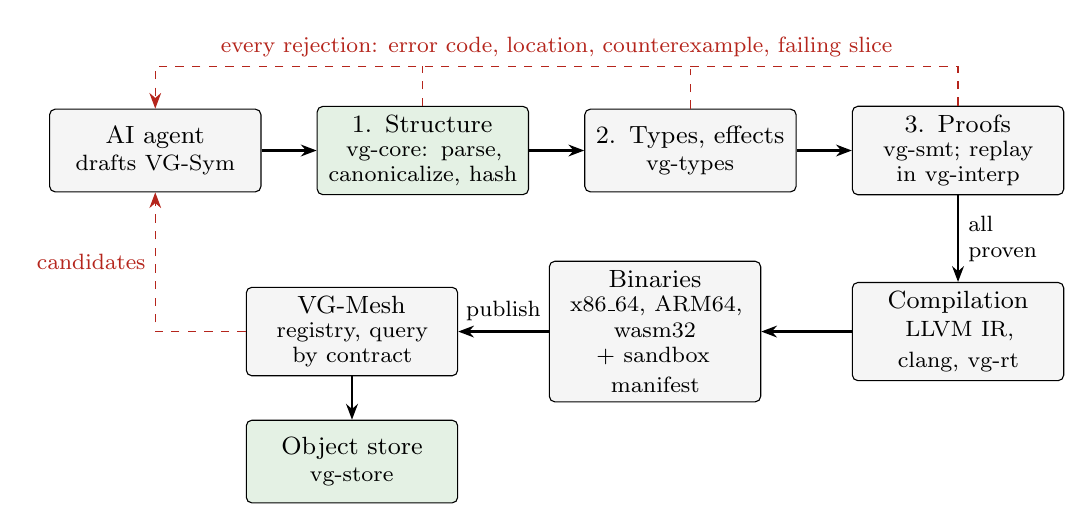
\begin{tikzpicture}[
  box/.style={draw, rounded corners=2pt, align=center, font=\small, minimum height=1.05cm,
              text width=2.45cm, fill=gray!8},
  built/.style={box, fill=ForestGreen!12},
  arr/.style={-{Stealth[length=2mm]}, thick},
  back/.style={-{Stealth[length=2mm]}, dashed, BrickRed},
  node distance=1.1cm and 0.7cm]
\node[box] (agent) {AI agent\\[-1pt]\footnotesize drafts VG-Sym};
\node[built, right=of agent] (struct) {1. Structure\\[-1pt]\footnotesize vg-core: parse,\\[-2pt]\footnotesize canonicalize, hash};
\node[box, right=of struct] (types) {2. Types, effects\\[-1pt]\footnotesize vg-types};
\node[box, right=of types] (proofs) {3. Proofs\\[-1pt]\footnotesize vg-smt; replay\\[-2pt]\footnotesize in vg-interp};
\node[box, below=of proofs] (codegen) {Compilation\\[-1pt]\footnotesize LLVM IR, clang, vg-rt};
\node[box, left=1.15cm of codegen] (bin) {Binaries\\[-1pt]\footnotesize x86\_64, ARM64, wasm32\\[-2pt]\footnotesize + sandbox manifest};
\node[box, left=1.15cm of bin] (mesh) {VG-Mesh\\[-1pt]\footnotesize registry, query\\[-2pt]\footnotesize by contract};
\node[built, below=0.55cm of mesh] (store) {Object store\\[-1pt]\footnotesize vg-store};
\draw[arr] (agent) -- (struct);
\draw[arr] (struct) -- (types);
\draw[arr] (types) -- (proofs);
\draw[arr] (proofs) -- node[right, font=\footnotesize, align=left] {all\\proven} (codegen);
\draw[arr] (codegen) -- (bin);
\draw[arr] (bin) -- node[above, font=\footnotesize] {publish} (mesh);
\draw[arr] (mesh) -- (store);
\draw[back] (proofs.north) -- ++(0,0.5) -| node[pos=0.25, above, font=\footnotesize]
  {every rejection: error code, location, counterexample, failing slice} (agent.north);
\draw[dashed, BrickRed] (struct.north) -- ++(0,0.5);
\draw[dashed, BrickRed] (types.north) -- ++(0,0.5);
\draw[back] (mesh.west) -| node[pos=0.75, left, font=\footnotesize] {candidates} (agent.south);
\end{tikzpicture}
\caption{The checking pipeline. Every draft passes structure, then types and effects, then
proofs; every rejection returns to the agent as structured data. Shaded green: implemented at
commit \texttt{fe499c8}; grey: specified, not implemented.}
\label{fig:pipeline}
\end{figure}

\Cref{fig:pipeline} shows the path from a draft to a binary. Each stage is a check whose
rejections return to the agent as typed JSON with stable codes, located in the agent's own
names: structural errors from vg-core, type and effect errors from vg-types, and, from vg-smt,
a verdict per obligation. A refutation carries a counterexample that the reference
interpreter must replay, and the part of the graph that the violation depends on. Agents may
also query the registry by contract before drafting. Only verified graphs reach code
generation.

\subsection{The counterexample-and-repair story}

The first draft of \kw{@soft\_knee} computed $u = t/(1+t)$ instead of $u = 1-1/(1+t)$
(\file{examples/soft\_knee\_draft.vgs}). For $x = 3\cdot 10^{38}$ and $\mathit{knee} = 0.5$ the
excess $t$ overflows to $+\infty$, the quotient $\infty/\infty$ is NaN, every later op
propagates it, and the first conjunct of \kw{POST}, \kw{result >= -1.0}, is false. The repaired
form is exactly $1$ at $t = +\infty$. The project's first milestone requires the verifier to
reject the draft with a counterexample that replays and to prove the repair.
\Cref{sec:case} proves both facts by hand, characterizes the failing inputs exactly, and
checks both claims by exhaustive enumeration.

\subsection{Design invariants}\label{sec:invariants}

The specification states eight invariants that follow from designing for agents; a change
that breaks one needs a recorded decision. We paraphrase them, because the formal results
below are about them.
\begin{enumerate}[label=(I\arabic*)]
\item \emph{Every judgment is data}: errors, verdicts, counterexamples and costs are typed
  JSON with stable codes.
\item \emph{Local reasoning}: types follow from operands, one op at a time, and a node is
  verified against its callees' contracts, never their bodies.
\item \emph{Prefix-checkable text}: ports and labels are defined before use, so every prefix
  of a file can be checked and a constrained decoder can mask by type.
\item \emph{Identity by content}: one canonical graph has one hash on every machine, so each
  obligation is proven once and the proof is reusable.
\item \emph{Same input, same bytes}: hashes, proofs, diagnostics, binaries and NaN bits are
  deterministic.
\item \emph{Nothing implicit}: no implicit conversion, no default arithmetic mode, no undefined
  behaviour in verified code, no inline expression.
\item \emph{Contracts are the shared language} between humans, agents, the verifier and the
  registry.
\item \emph{Honest guarantees}: an unknown solver answer is never a proof, a measurement is
  never a proof, and every guarantee names what it trusts.
\end{enumerate}

\subsection{What the specification corrected}

\VG{}'s specification began as a visionary source document. The current specification keeps
its goals and records 27 technical errors in it, each with a fix. Four fixes shape this paper.
First, the source let models write hashes, including invented ``built-in'' ones; now models
write labels and the toolchain computes hashes. Second, the source claimed that SHA-256 lifted
from two languages would converge to the same hash; structurally different implementations
cannot share a structural hash, and \cref{thm:conp} shows that no efficient canonical form
could make them do so in general, so implementations proven to refine one reference
specification join a \emph{spec class} instead. Third, the source assumed that every model
exposes per-token logit masking; hosted models do not, so they use a generate, verify and
repair loop through tools, and masking is reserved for local open-weight models. Fourth, the
source stated wall-clock latency as an SMT-provable postcondition; latency is now a measured
budget and only abstract costs are proven.

\section{A core calculus for \VG{} nodes}\label{sec:calculus}

This section fixes the objects the later theorems are about. The calculus covers the MVP
fragment of the specification: scalar, collection and float operations, the bounded
combinators \op{SIMD\_MAP}, \op{FOLD\_BOUNDED}, \op{GENERATE} and \op{ASSERT\_GUARD}, calls by
hash, and three effect operations. It leaves out what the MVP rejects: recursion, sum types,
generics and explicit memory regions. Individual operations are given by a table
(\cref{app:ops}); the calculus needs only their typing, domain and meaning.

\subsection{Types and values}

\begin{definition}[Types]\label{def:types}
\[
\begin{array}{rcl}
\tau & ::= & \mathsf{Bool} \mid \mathsf{u}N \mid \mathsf{i}N \mid \mathsf{f16} \mid
  \mathsf{bf16} \mid \mathsf{f32} \mid \mathsf{f64}
  \mid \mathsf{Array}\langle\tau, n\rangle \mid \mathsf{Tensor}\langle\tau,[d_1,\dots,d_k]\rangle
  \mid \mathsf{Slice}\langle\tau\rangle \\
  & \mid & \mathsf{Tuple}\langle\tau_1,\dots,\tau_k\rangle \mid
  \mathsf{Result}\langle\tau,\tau'\rangle \mid \Eff \mid \mathsf{FileIn} \mid \mathsf{FileOut}
  \mid \mathsf{Clock}
\end{array}
\]
with $N\in\{8,16,32,64\}$ and static $n, d_i$. A type is \emph{fixed-size} if it is
$\mathsf{Bool}$, a scalar, or an array, tensor, tuple or result built from fixed-size types.
\end{definition}

$\sem{\mathsf{u}N} = \{0,\dots,2^N-1\}$ and $\sem{\mathsf{i}N}=\{-2^{N-1},\dots,2^{N-1}-1\}$;
arrays, tensors and slices denote sequences (a slice of length below $2^{64}$), tuples and
results the usual products and tagged sums, $\sem{\Eff}=\{\star\}$, and handle types denote
opaque capabilities that only the runtime creates.

\begin{definition}[Float values with one NaN]\label{def:onenan}
Let $\varphi$ be one of the binary formats binary16, bfloat16, binary32 or binary64, of width
$w_\varphi$ bits. Let $\mathrm{Fin}_\varphi$ be its finite values, with $+0$ and $-0$ distinct,
and $V_\varphi = \mathrm{Fin}_\varphi \cup \{+\infty,-\infty,\NaN\}$. Let
$B_\varphi = \{0,1\}^{w_\varphi}$ be the bit patterns. The decoding
$\dec_\varphi : B_\varphi\to V_\varphi$ is the IEEE~754 decoding~\cite{ieee754-2019}, except
that every pattern with an all-ones exponent field and a non-zero significand decodes to the
single value $\NaN$. The encoding $\enc_\varphi : V_\varphi\to B_\varphi$ maps every non-NaN
value to its IEEE~754 encoding and $\NaN$ to the canonical quiet NaN $c_\varphi$ with a zero
sign bit: \texttt{0x7E00}, \texttt{0x7FC0}, \texttt{0x7FC00000} and
\texttt{0x7FF8000000000000} for the four formats. We write $\sem{\mathsf{f}N}=V_\varphi$.
\end{definition}

This is the float domain of the SMT-LIB theory of floating point~\cite{brain2015fp}, which has
a single NaN, and the NaN that the deterministic profile of WebAssembly
produces~\cite{wasm-spec}.

\begin{lemma}[Encoding and decoding]\label{lem:encdec}
$\dec_\varphi\circ\enc_\varphi=\mathrm{id}_{V_\varphi}$, and $\enc_\varphi\circ\dec_\varphi$ is
idempotent and fixes exactly the bit patterns that are not non-canonical NaNs. In particular
$\enc_\varphi$ is injective.
\end{lemma}
\begin{proof}
Binary interchange formats encode every non-NaN datum, each signed zero and each infinity by
exactly one bit pattern~\cite{ieee754-2019}; decimal formats, which have several encodings per
value, are not used. Hence $\dec(\enc(v))=v$ for $v\neq\NaN$, and $\dec(c_\varphi)=\NaN$. For a
pattern $p$, $\enc(\dec(p))=p$ unless $p$ encodes a NaN other than $c_\varphi$, in which case it
is $c_\varphi$; applying $\enc\circ\dec$ again changes nothing. Injectivity follows from the
left inverse.
\end{proof}

\subsection{Nodes}

\begin{definition}[Op symbols]\label{def:opsym}
An \emph{op symbol} $f$ is an opcode with its mode byte, its operand types
$(\tau_1,\dots,\tau_{n})$ and its result types $(\rho_1,\dots,\rho_{r})$. A \emph{primitive}
op symbol has a domain $D_f\subseteq\sem{\tau_1}\times\dots\times\sem{\tau_n}$ and a meaning
$\sem{f}: D_f\to\sem{\rho_1}\times\dots\times\sem{\rho_r}$; it is \emph{total} when $D_f$ is the
whole product. A set $\mathit{Comm}$ of binary op symbols is designated commutative
(\op{ADD}, \op{MUL}, \op{AND}, \op{OR}, \op{XOR}, \op{EQ}, \op{NE}, \op{BAND}, \op{BOR},
\op{FADD}, \op{FMUL}, \op{FMIN}, \op{FMAX}), and \op{FMA} is commutative in its first two
operands. \emph{Call-like} op symbols (\op{CALL\_HASH}, \op{ASSERT\_GUARD}, \op{SIMD\_MAP},
\op{FOLD\_BOUNDED}, \op{GENERATE}) take callee operands; \emph{effect} op symbols
(\op{FILE\_READ}, \op{FILE\_WRITE}, \op{CLOCK\_READ}) take an $\Eff$ token first and return one
first.
\end{definition}

The domain of a partial primitive op is its \emph{obligation} in the specification: for
example $D_{\op{ADD.checked}}$ contains the pairs whose exact sum fits the type,
$D_{\op{INDEX}}$ the pairs $(xs,i)$ with $i<\mathrm{len}(xs)$, and $D_{\op{FCOPYSIGN}}$ the
pairs whose second operand is not $\NaN$ (\cref{sec:float}).

\begin{definition}[Nodes]\label{def:node}
A node is a tuple $N=\langle P,\Theta,R,\varepsilon,(o_0,\dots,o_{k-1}),\mathit{out},C\rangle$
where $P=(\tau_1,\dots,\tau_m)$ are the parameter types;
$\Theta=((\varphi_1,lo_1,hi_1),\dots,(\varphi_l,lo_l,hi_l))$ are the learnable parameters, each
with a float format and bounds; the \emph{inputs} of $N$ are its parameters followed by its
learnable parameters, numbered $0,\dots,m+l-1$; $R=(\rho_1,\dots,\rho_r)$ are the result types;
$\varepsilon$ is a subset of the twelve effect names (\textsf{ARENA}, \textsf{CLOCK},
\textsf{FILE\_READ}, \textsf{FILE\_WRITE}, \dots); each op is $o_i=f_i(a_{i,1},\dots,a_{i,n_i})$
with operands
\[
a ::= \mathsf{in}(j) \mid \mathsf{const}(c) \mid \mathsf{callee}(h) \mid \mathsf{inv}(h) \mid
\mathsf{op}(i',s),
\]
denoting an input, a typed constant, the hash of a callee node, an invariant clause, and the
$s$-th result of op $o_{i'}$; $\mathit{out}=(a_1,\dots,a_r)$ are the output operands; and $C$
is the contract (\cref{sec:contracts}).
\end{definition}

\begin{definition}[Well-formed nodes]\label{def:wf}
A node is well formed when:
\begin{enumerate}[label=(W\arabic*),ref=W\arabic*]
\item\label{wf:order} \emph{Order.} Every operand $\mathsf{op}(i',s)$ of $o_i$ has $i'<i$ and
  $s$ below the number of results of $o_{i'}$, and an invariant never names a port that
  depends on the fold that uses it. Hence the op graph is acyclic and every port is defined
  before use.
\item\label{wf:typing} \emph{Local typing.} Operand types match the op symbol, and output
  types match $R$.
\item\label{wf:eff} \emph{Linear effect token.} If $\varepsilon\not\subseteq\{\textsf{ARENA}\}$,
  then input $0$ and result $0$ have type $\Eff$ and no other input or result has; otherwise no
  input or result has type $\Eff$. Each $\Eff$ value (input~$0$, and the $\Eff$ result of each
  op that returns one) is used exactly once in total, by the operands of ops and by
  $\mathit{out}$.
\item\label{wf:kernel} \emph{Kernels.} The callees of \op{SIMD\_MAP}, \op{FOLD\_BOUNDED} and
  \op{GENERATE} have an empty effect set, fixed-size parameter and result types, and one
  result.
\item\label{wf:effects} \emph{Effects.} An effect op occurs only if its effect is in
  $\varepsilon$, and $\varepsilon_g\subseteq\varepsilon$ for every callee $g$.
\item\label{wf:handles} \emph{Handles.} Values of type $\Eff$ or of a handle type occur only as
  top-level inputs and results, as call arguments and results, and as effect-op operands; never
  inside a tuple, result or collection, in a kernel signature, or as a constant.
\item\label{wf:calls} \emph{Calls.} The call graph is acyclic.
\item\label{wf:capacity} \emph{Field capacity.} Every count stored in a fixed-width field of
  the binary format fits that field (\cref{cond:capacity}).
\end{enumerate}
\end{definition}

The first property is what the specification calls define-before-use; it makes every prefix
of a VG-Sym file checkable (invariant~I3). The next lemma is the formal content of the
statement that the effect token ``orders'' effects.

Kernels are pure, but the callees of \op{ASSERT\_GUARD} are ordinary nodes and may have
effects. Such a guard takes the effect token as an argument and returns its selected callee's
token, so, like a call to an effectful node, it consumes one $\Eff$ value and produces one; only
the selected callee's effects happen.

\begin{lemma}[The effect chain]\label{lem:chain}
Let $N$ be well formed with $\varepsilon\not\subseteq\{\textsf{ARENA}\}$. The ops that consume
an $\Eff$ value form a single sequence $e_1,\dots,e_p$ such that $e_1$ consumes input $0$,
$e_{q+1}$ consumes the $\Eff$ result of $e_q$, and output $0$ is the $\Eff$ result of $e_p$
(or input $0$ when $p=0$). Hence the effectful ops of $N$, including calls to effectful nodes,
are totally ordered.
\end{lemma}
\begin{proof}
Let $G$ be the directed graph whose vertices are the $\Eff$ values of $N$, with an edge
$u\to w$ when the op that produces $w$ consumes $u$. Every op that consumes an $\Eff$ value
consumes exactly one and produces exactly one (\ref{wf:typing}, \ref{wf:eff}), so every vertex
other than input $0$ has in-degree exactly $1$, and input $0$ has in-degree $0$. Every vertex
is used exactly once (\ref{wf:eff}): either by an op, giving out-degree $1$, or by
$\mathit{out}$, giving out-degree $0$; since only result $0$ has type $\Eff$, exactly one
vertex is used by $\mathit{out}$. By \ref{wf:order} $G$ is acyclic. A finite acyclic graph
whose vertices all have in- and out-degree at most $1$ is a disjoint union of paths, one per
vertex of in-degree $0$; here there is one. So $G$ is a single path from input $0$ to the
vertex used by $\mathit{out}$, and it contains every $\Eff$ value. Listing the producers of
its vertices in path order gives $e_1,\dots,e_p$.
\end{proof}

\subsection{Evaluation}

\begin{definition}[Environment]\label{def:env}
An environment consists of a callee semantics $\eta$ and an effect trace $T=(t_1,t_2,\dots)$,
the sequence of value results that the environment supplies to effect ops. $\eta$ maps each
callee hash to a partial function; for an effectful callee, the function also takes the unread
rest of the trace and returns the part it has not read.
\end{definition}

\begin{definition}[Evaluation]\label{def:eval}
Fix a well-formed node $N$, an input vector $v$ and an environment $(\eta,T)$. The partial
function $\val$ on operands is defined by recursion on the op index, which \ref{wf:order}
makes well founded: $\val(\mathsf{in}(j))=v_j$, $\val(\mathsf{const}(c))=c$, and
$\val(\mathsf{op}(i,s))=\pi_s(\mathit{Res}_i)$, where the results $\mathit{Res}_i$ of $o_i$
are, writing $\bar a$ for the values of its operands:
\begin{itemize}
\item for a primitive op, $\sem{f_i}(\bar a)$ if $\bar a\in D_{f_i}$;
\item for $\op{CALL\_HASH}(\mathsf{callee}(h),\bar a)$, the value $\eta(h)(\bar a)$;
\item for $\op{ASSERT\_GUARD}(c,\mathsf{callee}(h_1),\bar a,\mathsf{callee}(h_2))$, the value
  $\eta(h_1)(\bar a)$ if $c=\true$ and $\eta(h_2)(\bar a)$ otherwise; only the selected callee
  is applied;
\item for $\op{SIMD\_MAP}(\mathsf{callee}(h),xs,\bar b)$, the collection $ys$ of the same shape
  with $ys[\iota]=\eta(h)(xs[\iota],\bar b)$ for every index $\iota$;
\item for $\op{FOLD\_BOUNDED}(\mathsf{callee}(h),xs,\bar b,\mathit{init})$, the value
  $\mathit{acc}_n$ where $n=\mathrm{len}(xs)$, $\mathit{acc}_0=\mathit{init}$ and
  $\mathit{acc}_{q+1}=\eta(h)(\mathit{acc}_q,xs[q],\bar b)$;
\item for $\op{GENERATE}(\mathsf{callee}(h),n,\bar b)$, the sequence $ys$ with
  $ys[q]=\eta(h)(q,\bar b)$ for $q<n$;
\item for the ops on the effect chain of \cref{lem:chain}, taken in chain order: an effect op
  receives the pair $(\star,t)$, where $t$ is the next unread entry of $T$, and a call, or a
  guard whose selected callee is effectful, passes the unread rest of $T$ to that callee, which
  reads its own entries in the same way;
\end{itemize}
and $\mathit{Res}_i$ is undefined, a \emph{trap}, when an operand value is undefined, lies
outside the domain, or a required callee application is undefined. $N$ \emph{traps} on
$(v,\eta,T)$ when some $\mathit{Res}_i$ is undefined; otherwise its result is
$(\val(a_1),\dots,\val(a_r))$ for $\mathit{out}=(a_1,\dots,a_r)$.
\end{definition}

Evaluation is strict: every op is evaluated whether or not its value is used, and
\op{ASSERT\_GUARD} is the only op that applies one callee and not the other. The meaning of a
VG-Sym text is the meaning of its canonical node (\cref{sec:identity}), from which dead ops have
been removed; a dead partial op therefore never traps.

\begin{proposition}[Determinism]\label{prop:determinism}
The result of $N$ on $(v,\eta,T)$, or the fact that it traps, is uniquely determined by
$(v,\eta,T)$. Every evaluation order that respects data dependencies computes the same values.
\end{proposition}
\begin{proof}
\Cref{def:eval} defines $\val$ by well-founded recursion, so it is a function. The value of
each op depends only on the values of its operands, which precede it. The trace entries an
effect op receives are fixed by the order of the effect chain, a property of the graph that
\cref{lem:chain} makes well defined, and, by induction on the call graph, by the same property
of the callees on the chain; they do not depend on the order in which pure ops are executed.
\end{proof}

\subsection{Contracts}\label{sec:contracts}

Contract formulas are a small logic over the same values. Terms name inputs by position,
\kw{result} and \kw{result.j}, ports (in invariants only), bound variables, and typed
constants; they combine them with integer arithmetic over $\Z$ (no wrapping), float
arithmetic rounded to nearest-even, IEEE comparisons, the Boolean connectives,
indexing, projection, bounded quantification $\kw{forall}(i\ \kw{in}\ a..b)\,\{\phi\}$
(over the integers $a\le i<b$), the built-ins \kw{len}, \kw{is\_finite}, \kw{is\_nan},
\kw{abs}, \kw{min}, \kw{max}, \kw{as\_bytes}, \kw{same}, \kw{is\_ok}, \kw{ok}, \kw{err}, the
fold term $\kw{fold:}f(\mathit{init},xs,k,\bar b)$, the specification call
$\kw{spec:}s(\bar t)$ and kernel applications. On floats, \kw{==} is IEEE equality
($\NaN\neq\NaN$, $-0=+0$) and $\kw{same}(a,b)$ is identity.

\begin{definition}[Unspecified values]\label{def:unspecified}
An \emph{interpretation} $\iota$ assigns a value to every application outside its domain:
integer division or remainder by zero, out-of-range indexing, \kw{ok} of an error and \kw{err}
of a success, $\kw{spec:}s$ outside the precondition of $s$, $\kw{fold:}f$ with $k$ outside
$[0,\mathrm{len}(xs)]$, and an op outside its domain inside a kernel applied in a formula. We write
$\sem{\phi}^\iota_\sigma$ for the value of $\phi$ under an assignment $\sigma$ of inputs,
results and ports, and under $\iota$.
\end{definition}

Quantifying over every $\iota$ is how ``unspecified'' is made precise: no proof can depend on
an unspecified value, because it must hold for every choice of it.

\begin{definition}[Satisfying a contract]\label{def:satisfies}
Let $\mathit{Box}(v)$ state that each learnable input lies within its bounds. A node $N$
\emph{satisfies its contract} if for every input $v$ with $\mathit{Box}(v)$, every
interpretation $\iota$ with $\sem{\Pre}^\iota_v=\true$, every admissible trace $T$, and the
callee semantics of the nodes $N$ calls: $N$ does not trap on $(v,\eta,T)$, its result $y$
satisfies $\sem{\Post}^\iota_{v,y}=\true$, and the invariant of every \op{FOLD\_BOUNDED} holds
at every step of that fold.
\end{definition}

A trace is admissible when it respects the environment facts the specification states, such
as the monotonicity of successive clock reads along one chain.

The specification also requires contracts to be \emph{well defined}: each term that could
read an unspecified value adds an obligation saying that it does not, proven in the context
where the term occurs (under the left operand of \kw{\&\&} for its right operand, under the
negated left operand of \kw{||}, under the antecedent of \kw{==>}, under the range bounds
inside \kw{forall}). Write $\mathit{WD}(\phi)$ for the conjunction of these conditions.

\begin{lemma}[Well-defined formulas have one value]\label{lem:wd}
If $\sem{\mathit{WD}(\phi)}^\iota_\sigma=\true$ for every $\iota$, then
$\sem{\phi}^\iota_\sigma=\sem{\phi}^{\iota'}_\sigma$ for all $\iota,\iota'$.
\end{lemma}
\begin{proof}
By induction on $\phi$. Variables and constants do not depend on $\iota$. For an application
$p(t_1,\dots,t_n)$ that may leave its domain, $\mathit{WD}$ contains $\mathit{WD}(t_k)$ for each
$k$ and the domain condition of $p$; by induction the arguments have $\iota$-independent values,
and they lie in the domain, where $p$ is not interpreted by $\iota$. For $t_1\mathbin{\&\&}t_2$,
$\mathit{WD}$ is $\mathit{WD}(t_1)\wedge(t_1\Rightarrow\mathit{WD}(t_2))$: $t_1$ has an
$\iota$-independent value; if it is false, so is the conjunction for every $\iota$; if it is
true, $\mathit{WD}(t_2)$ holds for every $\iota$ and the induction hypothesis applies to $t_2$.
The cases of \kw{||} and \kw{==>} are symmetric. For $\kw{forall}(i\ \kw{in}\ a..b)\{\psi\}$,
$\mathit{WD}$ contains $\mathit{WD}(a)$, $\mathit{WD}(b)$ and $\mathit{WD}(\psi)$ for every
integer $i$ in the range, so the range and every instance have $\iota$-independent values.
\end{proof}

\subsection{Effects and capabilities}

Effect sets are ordered by inclusion; the empty set is \emph{pure} and union is the join. The
specification enforces \ref{wf:effects} at every call and counts kernels as callees.

\begin{proposition}[Effect containment]\label{prop:effects}
Let every node of a program be well formed. During any evaluation of a node $N$, including the
evaluations of its callees, every effect op that executes has its effect in $\varepsilon_N$.
\end{proposition}
\begin{proof}
By induction on the height of $N$ in the call graph, which is acyclic (\ref{wf:calls}). Effect
ops in the body of $N$ have their effect in $\varepsilon_N$ by \ref{wf:effects}. An effect op
executed inside a callee $g$ has its effect in $\varepsilon_g$ by induction, and
$\varepsilon_g\subseteq\varepsilon_N$ by \ref{wf:effects}. Kernels have empty effect sets
(\ref{wf:kernel}).
\end{proof}

\begin{proposition}[No forged capabilities]\label{prop:caps}
Let every node of a program be well formed, and let a root node be called with handles opened
by the runtime. Every handle that an effect op receives during the evaluation is one of those
handles.
\end{proposition}
\begin{proof}
We show by induction on the height of a node $N$ in the call graph that every handle value
occurring in an evaluation of $N$ is one of the handle values among the inputs of $N$. A handle
value in the body of $N$ is the value of an operand of handle type. Constants have no handle
type and no primitive or effect op has a handle result (\ref{wf:handles},
\cref{app:ops}), and handles cannot be stored in or projected out of tuples, results or
collections (\ref{wf:handles}). So the operand is an input of $N$, or a result of a call whose
handle results are, by induction, handle inputs of the callee, that is, handle arguments
supplied by $N$, which are themselves operands of $N$ of handle type. Induction on the op
index closes the argument. For the root, the inputs are the handles the runtime opened.
\end{proof}

The specification extends this confinement to the whole process: the runtime opens the
handles named by the root's manifest, then drops every other authority through Landlock and
seccomp on Linux, a generated sandbox profile on macOS, and preopened directories under WASI.
That step relies on the operating system and is outside the scope of our proofs.

\section{Identity: canonical forms and content addressing}\label{sec:identity}

A \VG{} node is named by hashes. The \emph{body hash} covers the op graph, the \emph{contract
hash} the canonical contract, and the \emph{node hash} the format version, the effect set,
the signature and the other two. All are BLAKE3 hashes in derive-key mode, one context string
per kind of hash, so hashes of different kinds are computed by different keyed functions. This
section characterizes exactly when two bodies share a hash, shows that a shared node hash
implies a shared meaning, and explains why semantic equivalence needs a different mechanism.

\subsection{Canonicalization}

The specification canonicalizes a node in seven steps: validate the structure; resolve labels
to hashes and drop identity ops and debug information; hash bottom-up; sort the operands of
commutative ops by hash; merge ops with equal hashes and drop ops on which no output, effect
chain or live invariant depends; number the remaining ops by a post-order depth-first walk
from the outputs, in port order; serialize the sections deterministically. The hash of an op
covers its opcode, mode, attribute word, result types and the hashes of its operands in port
order, after the commutative sort. An input hashes as its position and type, a constant as its
type and exact bytes, a callee as its node hash, and an op result as its op's hash and its
result index.

\subsection{Terms and unraveling}

\begin{definition}[Terms]\label{def:terms}
\emph{Operand terms} $t$ and \emph{op terms} $u$ are given by
\[
t ::= \mathsf{in}(j,\tau) \mid \mathsf{const}(\tau,b) \mid \mathsf{callee}(h) \mid
      \mathsf{inv}(h) \mid \langle u\rangle_s
\qquad\qquad
u ::= f(t_1,\dots,t_n),
\]
where $b$ is a byte string, $h$ a hash, $s$ a result index and $f$ an op symbol of arity $n$.
The \emph{unraveling} $\unr$ of an operand of a well-formed node is defined by recursion on the
op index: $\unr(\mathsf{in}(j))=\mathsf{in}(j,\tau_j)$,
$\unr(\mathsf{const}(c))=\mathsf{const}(\tau_c,\enc(c))$,
$\unr(\mathsf{callee}(h))=\mathsf{callee}(h)$, $\unr(\mathsf{inv}(h))=\mathsf{inv}(h)$, and
$\unr(\mathsf{op}(i,s))=\langle f_i(\unr(a_{i,1}),\dots,\unr(a_{i,n_i}))\rangle_s$.
\end{definition}

Unraveling forgets sharing: a body is a term graph~\cite{ariola1996equational}, and its
unraveling is the tuple of trees it denotes.

\begin{definition}[Equality up to commutativity]\label{def:eqc}
$\eqC$ is the least congruence on terms that contains $f(t_1,t_2)\eqC f(t_2,t_1)$ for every
$f\in\mathit{Comm}$ and $\op{FMA}(t_1,t_2,t_3)\eqC\op{FMA}(t_2,t_1,t_3)$.
\end{definition}

\subsection{Structural encodings and the capacity condition}

Every hash is computed from a byte string, its \emph{preimage}, built from fixed-width
integers, 32-byte hashes and type encodings. A type is encoded as a tag byte, an argument-count
byte, and its arguments, each of which is either a nested type encoding or a 32-bit immediate
(a bit width, an array length, a tensor dimension or a handle kind); the tag determines which.
The preimages hashed under the op context are
\begin{align*}
\pre(\mathsf{in}(j,\tau)) &= \mathtt{00}\cat u_{32}(j)\cat\enc_T(\tau) &
\pre(\mathsf{callee}(h)) &= \mathtt{03}\cat h \\
\pre(\langle u\rangle_s) &= \mathtt{01}\cat\Hop(\pre(u))\cat u_8(s) &
\pre(\mathsf{inv}(h)) &= \mathtt{04}\cat h \\
\pre(\mathsf{const}(\tau,b)) &= \mathtt{02}\cat\enc_T(\tau)\cat u_{32}(|b|)\cat b
\end{align*}
\begin{align*}
\pre(f(t_1,\dots,t_n)) = {}& \mathtt{05}\cat u_{16}(\mathit{opcode})\cat u_8(\mathit{mode})\cat
  u_{32}(\mathit{attr})\cat u_8(r)\cat\enc_T(\rho_1)\cat\dots\cat\enc_T(\rho_r)\\
  & {}\cat u_{32}(n)\cat h_{\pi(1)}\cat\dots\cat h_{\pi(n)},
\end{align*}
where $h_k=\Hop(\pre(t_k))$ and the permutation $\pi$ sorts the commutative positions
($\{1,2\}$ for $f\in\mathit{Comm}$ or $f=\op{FMA}$) by increasing byte string and fixes the
others. We write $\hash(t)=\Hop(\pre(t))$. Ties in the sort are harmless: two operands with the
same hash contribute the same bytes in either order. The hash of an invariant covers the ports
it names through their operand hashes; since an invariant never names a port that depends on the
fold that uses it (\ref{wf:order}), these definitions are well founded. The prototype rejects a
violation with the message ``an INVARIANT names a port that depends on the fold that uses it''.

\begin{assumption}[Field capacity]\label{cond:capacity}
Every integer written into a $w$-bit field is below $2^w$. For the fields above this means: at
most 255 tuple members, at most 254 tensor dimensions (the argument count of a tensor is one
more than its number of dimensions), at most 255 results per op, and result indices below 256.
\end{assumption}

\begin{lemma}[Prefix-free encodings]\label{lem:prefixfree}
Under \cref{cond:capacity}, $\enc_T$ is prefix-free: no type encoding is a proper prefix of
another, and a concatenation of type encodings determines the sequence of types. Preimages of
different kinds differ in their first byte, and equal preimages have equal fields: the same
leaf; or the same op hash and result index; or the same op symbol, arity and sequence of operand
hashes.
\end{lemma}
\begin{proof}
For types, by induction on nesting depth. A decoder reads the tag, which fixes the kind of each
argument (for example, an array has a type and then an immediate, a tuple has only types); it
reads the count, which by \cref{cond:capacity} is the true number of arguments; and it reads
each argument, an immediate of four bytes or, by induction, a uniquely delimited type
encoding. So each encoding is parsed in exactly one way and ends at a determined position,
which excludes proper prefixes. For preimages, the first byte fixes the kind; the remaining
fields have fixed widths, are 32-byte hashes, or are type encodings, which are uniquely
delimited, and counts ($r$, $n$, $|b|$) are exact by \cref{cond:capacity}. So equal preimages
have equal fields.
\end{proof}

\begin{remark}[Why the condition is not a formality]\label{rem:capacity}
Without \cref{cond:capacity} the encoding is ambiguous. If the member count of a tuple is
written as one byte modulo 256, then $\mathsf{Tuple}\langle\mathsf{Tuple}\langle
\mathsf{u8}^{257}\rangle,\mathsf{u8}\rangle$ and
$\mathsf{Tuple}\langle\mathsf{Tuple}\langle\mathsf{u8}\rangle,\mathsf{u8}^{257}\rangle$ both
encode as $[\mathsf{TUPLE},2][\mathsf{TUPLE},1]$ followed by 258 copies of the encoding of
$\mathsf{u8}$, although they are different types. \Cref{sec:status} reports that the prototype
writes these counts without enforcing the bound, and that the two identity functions on these
types receive the same node hash.
\end{remark}

\subsection{The characterization theorem}

\begin{assumption}[Collision freeness]\label{ass:cr}
For each hash context, distinct preimages that occur have distinct hashes.
\end{assumption}

No hash function is collision free, but a 256-bit function makes collisions improbable, and
derive-key mode keeps contexts apart. The standard idealization quantifies this.

\begin{lemma}[Birthday bound]\label{lem:birthday}
Let $H$ be a uniformly random function into $\{0,1\}^{256}$. For any procedure that makes at
most $q$ distinct queries to $H$, possibly adaptively, the probability that two queries
collide is at most $q(q-1)/2^{257}$.
\end{lemma}
\begin{proof}
The $k$-th distinct query receives a uniformly random value independent of the previous ones,
so it collides with one of the $k-1$ earlier values with probability at most
$(k-1)/2^{256}$. Summing over $k\le q$ gives $q(q-1)/2^{257}$.
\end{proof}

For $q=2^{64}$ preimages the bound is about $2^{-129}$. Modelling each derive-key context of
BLAKE3 as an independent random function is a heuristic~\cite{bellare1993random}; BLAKE3 has a
256-bit output and is designed for a 128-bit security level~\cite{blake3}.
\Cref{ass:cr} is the event that no collision occurs.

\begin{theorem}[Hashes characterize terms up to commutativity]\label{thm:hash-char}
Assume \cref{cond:capacity,ass:cr}. For all operand terms $t,t'$ that arise from well-formed
nodes, $\hash(t)=\hash(t')$ if and only if $t\eqC t'$.
\end{theorem}
\begin{proof}
($\Leftarrow$) Let $t\sim t'$ mean $\hash(t)=\hash(t')$; it is an equivalence relation. It is a
congruence: if $t_k\sim t'_k$ for every $k$, the preimages of $f(t_1,\dots,t_n)$ and
$f(t'_1,\dots,t'_n)$ contain the same operand hashes, sorted the same way, so the op terms have
equal hashes, and so do $\langle f(\dots)\rangle_s$ and $\langle f(\dots)\rangle_s$ for every
$s$. It contains the generators of $\eqC$: for commutative positions, sorting
$(\hash(t_1),\hash(t_2))$ and $(\hash(t_2),\hash(t_1))$ yields the same sequence. Since $\eqC$
is the least congruence containing the generators, ${\eqC}\subseteq{\sim}$.

($\Rightarrow$) By induction on the sum of the sizes of $t$ and $t'$. Suppose
$\hash(t)=\hash(t')$. By \cref{ass:cr}, $\pre(t)=\pre(t')$, and by \cref{lem:prefixfree} $t$ and
$t'$ have the same kind and equal fields. If they are leaves, they are equal. Otherwise
$t=\langle u\rangle_s$ and $t'=\langle u'\rangle_{s}$ with $\Hop(\pre(u))=\Hop(\pre(u'))$, hence
$\pre(u)=\pre(u')$ by \cref{ass:cr}. By \cref{lem:prefixfree}, $u=f(t_1,\dots,t_n)$ and
$u'=f(t'_1,\dots,t'_n)$ have the same op symbol (opcode, mode, attribute and result types)
and the same arity, and their sorted operand-hash sequences are equal. At a non-commutative
position $k$, $\hash(t_k)=\hash(t'_k)$, so $t_k\eqC t'_k$ by induction. At the commutative
positions, the multisets $\{\hash(t_1),\hash(t_2)\}$ and $\{\hash(t'_1),\hash(t'_2)\}$ are
equal; so either $\hash(t_1)=\hash(t'_1)$ and $\hash(t_2)=\hash(t'_2)$, or
$\hash(t_1)=\hash(t'_2)$ and $\hash(t_2)=\hash(t'_1)$. In the first case $t_1\eqC t'_1$ and
$t_2\eqC t'_2$ by induction; in the second, $t_1\eqC t'_2$ and $t_2\eqC t'_1$, and
$f(t_1,t_2,\dots)\eqC f(t'_2,t'_1,\dots)\eqC f(t'_1,t'_2,\dots)$ by the commutativity
generator. Either way $u\eqC u'$, hence $t\eqC t'$.
\end{proof}

The body hash is computed under its own context from the output count, the hashes of the
output operands, and, for each learnable parameter, its type, its bounds as constants and the
hash of its loss node if it has one.

\begin{corollary}[Body hashes]\label{cor:body}
Under the assumptions of \cref{thm:hash-char}, two well-formed nodes have equal body hashes
if and only if they have the same number of outputs, $\unr(a_k)\eqC\unr(a'_k)$ for every output
$k$, and equal learnable boxes.
\end{corollary}

\begin{corollary}[Canonical form]\label{cor:canon}
Under the assumptions of \cref{thm:hash-char}, steps~5 and~6 of canonicalization merge two ops
exactly when their op terms are equal up to commutativity, and the canonical body is
determined by the $\eqC$-classes of the unraveled outputs and of the terms the live invariants
refer to. Consequently canonicalization is idempotent, and each of the following moves of the
specification leaves the canonical body unchanged: consistent renaming of ports, parameters,
bound variables and labels; reordering statements while respecting \ref{wf:order}; duplicating
a pure op; adding a pure op that nothing uses; swapping the operands of a commutative op;
binding a value through an identity op; and changing comments or debug text.
\end{corollary}
\begin{proof}
By \cref{thm:hash-char}, equal op hashes mean $\eqC$-equal op terms, so merging by hash
identifies exactly the $\eqC$-classes; the post-order numbering from the outputs, in port order
and with operands of commutative ops in sorted order, is then a function of the merged graph.
Hence the canonical body depends only on the classes named in the statement, and
canonicalizing it again finds the same classes. Each move preserves those classes: renaming
changes no position, hash or label resolution; reordering does not change $\unr$; a duplicate
of a pure op has the same term; an unused op contributes to no output term; a commutative swap
is a generator of $\eqC$; identity ops are erased before hashing; comments and debug text are
not hashed.
\end{proof}

The specification also states the converse: texts with equal canonical forms are related by
these moves. As listed, the moves do not suffice, because canonicalization makes three further
identifications that the specification states elsewhere: several clauses of one kind join into
one conjunction in source order; a refined parameter or result type is stored as its base type
with the refinement conjoined to the precondition or postcondition; and two literals that
denote the same value, such as \kw{0.99} and its binary32 rounding written out, or the integers
\kw{-0} and \kw{0}, are the same constant. With these three added to the moves, every text can be
moved to the canonical printing of its canonical form (the printer emits callees first and ops in
post-order, which respects \ref{wf:order}), and the moves can be reversed, which gives the
converse. We do not formalize the printer, so we state this direction as a remark rather than a
theorem.

\subsection{Effects are never merged}

Merging ops with equal hashes is sound for pure ops, whose copies and discards are
natural~\cite{fox1976coalgebras}; it would be wrong for effects, since two reads of a clock are
two observations. The specification's answer is the effect token; the next lemma shows that it
suffices.

\begin{lemma}[Effectful ops are never merged]\label{lem:eff-never-merged}
Assume \cref{cond:capacity,ass:cr}, and let $N$ satisfy \ref{wf:eff}. Distinct ops of $N$ that
consume an $\Eff$ value have distinct hashes. Hence step~5 never merges them.
\end{lemma}
\begin{proof}
By \cref{lem:chain}, these ops form the chain $e_1,\dots,e_p$. Let $\epsilon_0$ be input $0$
and $\epsilon_q$ the $\Eff$ result of $e_q$. Suppose $\hash(e_i)=\hash(e_j)$ with $i<j$. By
\cref{ass:cr} and \cref{lem:prefixfree} the two op terms have the same opcode, hence the same
operand layout, and equal operand hashes at every position, in particular at the position of
the $\Eff$ operand: $\hash(\epsilon_{i-1})=\hash(\epsilon_{j-1})$. If $i>1$, both are op results,
so their preimages are equal and $\hash(e_{i-1})=\hash(e_{j-1})$. Repeating $i-1$ times gives
$\hash(\epsilon_0)=\hash(\epsilon_{j-i})$ with $j-i\ge1$. But the preimage of $\epsilon_0$ starts
with byte \texttt{00} (an input) and that of $\epsilon_{j-i}$ with \texttt{01} (an op result),
so the preimages differ and \cref{ass:cr} is contradicted.
\end{proof}

The lemma depends on \ref{wf:eff}. A node in which one token feeds two effect ops cannot be
written in VG-Sym, because the text lowering rejects it, but it can be built through an API or
read from bytes. \Cref{sec:status} reports that the prototype's decoder accepts such a node
and that its merge step then merges two clock reads. The lemma shows that checking
\ref{wf:eff} on every path into the canonicalizer, the decoder included, restores the
guarantee.

\subsection{Equal hashes, equal meaning}

The meaning of an operand term is defined compositionally: $\sem{\mathsf{in}(j,\tau)}=v_j$,
constants denote their values, $\sem{\langle f(t_1,\dots,t_n)\rangle_s}$ applies the meaning of
$f$ (as in \cref{def:eval}) to the meanings of the $t_k$, and the ops on the effect chain read
the trace in the order in which their $\Eff$ operands are nested, which is the order of the
chain.

\begin{lemma}[Unraveling preserves meaning]\label{lem:unr-sem}
For every operand $a$ of a well-formed node, $\val(a)=\sem{\unr(a)}$, both sides being
undefined together.
\end{lemma}
\begin{proof}
By induction on the op index. The two definitions apply the same function to the same operand
values; for the ops on the effect chain, the order of the chain (\cref{lem:chain}) is the order
in which their $\Eff$ operands are nested in the terms, so both definitions hand them the same
trace entries.
\end{proof}

\begin{theorem}[Equal node hashes imply equal meaning]\label{thm:hash-meaning}
Assume \cref{cond:capacity,ass:cr}, and that callees with equal hashes have equal meanings. If
two well-formed canonical nodes $N$ and $N'$ have equal node hashes, then they have the same
format version, effect set, signature and learnable box; for every input, callee semantics and
trace, either both trap or both return the same result; and their contracts are equal up to
the renaming of parameters and bound variables.
\end{theorem}
\begin{proof}
By \cref{ass:cr} the node-hash preimages are equal, so the version, effect set, signature, box,
body hash and contract hash coincide. By \cref{cor:body}, the output terms are $\eqC$-equal. The
meaning of an op symbol in $\mathit{Comm}$ is a commutative function: obviously so for integers
and Booleans, and for floats by \cref{thm:float-comm} below; hence $\eqC$-equal terms have
equal meanings, traps included, by induction on the congruence. By \cref{lem:unr-sem} the
outputs of $N$ and $N'$ have equal values. Ops that only invariants use are covered by the
contract hash, which encodes each port by its operand hash, so their terms, and therefore their
traps, agree as well. Finally, the canonical contract encodes parameters by position and bound
variables by de Bruijn index~\cite{maziarz2021hashing}, so equal contract hashes mean equal
formulas up to renaming.
\end{proof}

Two artifacts with one node hash can still differ outside the node's meaning. The attributes
\kw{export} and \kw{inline} are not hashed, although \kw{export} makes the code generator emit a
checked entry point; the specification leaves that choice to the owner.

\subsection{Why semantic identity needs specifications}

The source document of \VG{} expected two implementations of SHA-256 to converge to one hash.
\Cref{thm:hash-char} shows that a structural hash cannot do this unless the implementations
unravel to the same terms. One might hope for a smarter canonical form. The next theorem shows
that no efficient one exists.

\begin{theorem}[Semantic equivalence is coNP-hard]\label{thm:conp}
Deciding whether two pure, fixed-size, well-formed nodes compute the same function is
coNP-hard, already for nodes with only Boolean inputs and the ops \op{BAND}, \op{BOR} and
\op{BNOT}.
\end{theorem}
\begin{proof}
We reduce the complement of satisfiability, which is coNP-complete~\cite{cook1971complexity},
to equivalence. Given a propositional formula $\psi$ over variables $p_1,\dots,p_n$, build the
node $N_\psi$ with signature $(\mathsf{Bool}^n)\to(\mathsf{Bool})$ that evaluates $\psi$ with
one \op{BAND}, \op{BOR} or \op{BNOT} per connective, and the node $N_\bot$ with the same
signature that returns the constant \kw{false}. Both are well formed and pure, and the
construction takes time linear in $|\psi|$. They compute the same function if and only if
$\psi$ is unsatisfiable.
\end{proof}

\begin{corollary}\label{cor:no-canon}
If some polynomial-time computable function $c$ on nodes satisfied $c(N)=c(N')$ exactly when
$N$ and $N'$ compute the same function, then $\mathrm{P}=\mathrm{NP}$.
\end{corollary}
\begin{proof}
Equivalence would be decidable in polynomial time by comparing $c(N_\psi)$ with $c(N_\bot)$,
so unsatisfiability would be in P, hence coNP $=$ P and therefore NP $=$ P.
\end{proof}

Any efficiently computable identity must therefore either merge some inequivalent programs or
separate some equivalent ones. \VG{} chooses the second, which is the safe failure, and handles
semantic identity by specification: a SPEC node is an executable reference, and an
implementation joins its spec class when its postcondition \kw{result == spec:s(\dots)} is
proven. The registry records how membership was shown: \emph{proved} for every input,
\emph{bounded}$(n)$ for inputs of size at most $n$, or \emph{tested}$(m)$ on $m$ cases, which a
caller's proof may never rely on.

\begin{proposition}[Spec classes are extensional]\label{prop:specclass}
Let $I_1$ and $I_2$ satisfy their contracts (\cref{def:satisfies}) with postconditions
$\kw{result == spec:}s(\bar x)$, for a result type on which \kw{==} is identity (integers,
Booleans and collections of them), and let $s$ satisfy its own contract. Then $I_1(\bar v)=
I_2(\bar v)$ for every $\bar v$ that satisfies the preconditions of $I_1$, $I_2$ and $s$.
\end{proposition}
\begin{proof}
For such $\bar v$, $\bar v$ lies in the domain of $\kw{spec:}s$, where the term denotes
$s(\bar v)$ in every interpretation. The postconditions of $I_1$ and $I_2$ hold at $\bar v$, so
$I_1(\bar v)=s(\bar v)=I_2(\bar v)$.
\end{proof}

For float results \kw{==} is IEEE equality, under which $-0=+0$ and $\NaN\neq\NaN$; a spec class
over floats must use \kw{same} to obtain the same conclusion.

\subsection{Short hashes}

Text and diagnostics show a hash as \texttt{\#} followed by 12 hexadecimal digits. If $n$
uniformly random 48-bit prefixes are drawn, a collision becomes more likely than not near
$n\approx\sqrt{2\ln 2\cdot 2^{48}}\approx 1.98\times10^{7}$; for 8 digits (32 bits) the same
estimate is about $7.7\times10^{4}$. The toolchain lengthens a displayed prefix on any clash
within a module, and binaries always carry all 32 bytes, so short hashes are a convenience,
never an identity.

\section{Floating point with one NaN}\label{sec:float}

The design promises that a node produces the same bytes in the interpreter and on x86\_64,
ARM64 and WebAssembly (invariant~I5). For floats this cannot hold at the level of bit patterns.
LLVM gives a NaN result a nondeterministic sign and a payload chosen among several
options~\cite{llvm-langref}; x86\_64 and AArch64 produce different default NaNs; WebAssembly is
deterministic only in its deterministic profile, which produces positive canonical
NaNs~\cite{wasm-spec}; and the SMT-LIB theory of floating point, in which the verifier reasons,
has a single NaN~\cite{brain2015fp}. \VG{} therefore gives floats the one-NaN domain of
\cref{def:onenan}: a float value is a number, an infinity or $\NaN$, and wherever a float
becomes bytes, $\NaN$ is written as the canonical NaN. This section proves that the choice is
coherent, and states exactly where it constrains the language.

\subsection{Operations descend to the quotient}

Write $p\sim q$ for bit patterns with $\dec(p)=\dec(q)$; the classes of $\sim$ are the values
$V_\varphi$. IEEE~754 lets an operation that returns a NaN choose among NaN patterns, so we read
each operation $g$ as a relation between operand patterns and admissible result patterns. We
say that $g$ \emph{descends to the quotient} on a set of operand values $D$ if there is a
function $\hat g : D\to V_\varphi$ (or into $\mathsf{Bool}$, or an integer type) such that
$\dec(z)=\hat g(\dec(p_1),\dots,\dec(p_n))$ for all operand patterns $p_k$ with
$(\dec(p_1),\dots,\dec(p_n))\in D$ and every admissible result $z$ of $g(p_1,\dots,p_n)$.

\begin{theorem}[One NaN is a congruence]\label{thm:float-congruence}
Every MVP float operation descends to the quotient on its whole domain, with one exception:
\op{FCOPYSIGN}$(x,y)$ descends exactly on the operand values with $y\neq\NaN$. The operations
covered are \op{FADD}, \op{FSUB}, \op{FMUL}, \op{FDIV}, \op{FMA}, \op{FSQRT}, \op{FNEG},
\op{FABS}, \op{FMIN}, \op{FMAX}, \op{FCLAMP}, \op{FCOPYSIGN}, the float comparisons, \op{CAST}
between float formats and between floats and integers, and \op{AS\_BYTES}.
\end{theorem}
\begin{proof}
A non-NaN value has exactly one pattern (\cref{lem:encdec}), so patterns in one class can
differ only when the class is $\NaN$. It suffices to check, for each operation, that the class
of the result does not depend on which NaN pattern an operand carries.
\begin{enumerate}[label=(\alph*)]
\item \op{FADD}, \op{FSUB}, \op{FMUL}, \op{FDIV}, \op{FMA}, \op{FSQRT} and conversions between
  formats are general-computational operations. If an operand is a NaN, the result is a quiet
  NaN; otherwise the result is the correctly rounded exact result, or a NaN for an invalid
  operation ($\infty-\infty$, $0\cdot\infty$, $0/0$, $\infty/\infty$, the square root of a
  negative number), or a signed infinity on overflow or division by zero~\cite{ieee754-2019}.
  In every case the class of the result is a function of the operand values.
\item \op{FMIN} and \op{FMAX} are the operations \emph{minimum} and \emph{maximum} of IEEE
  754-2019: the result is a NaN if either operand is a NaN, and otherwise the lesser (greater)
  operand, with $-0<+0$. They are not the NaN-avoiding operations \emph{minNum} of IEEE
  754-2008 or \emph{minimumNumber} of IEEE 754-2019, which return the other operand when one
  is a NaN.
\item The comparisons are false for $<,\le,>,\ge,=$ and true for $\neq$ when an operand is a NaN,
  and otherwise depend only on the values.
\item \op{FNEG} and \op{FABS} are bit operations on the sign; they map NaN patterns to NaN
  patterns and non-NaN values to determined values.
\item \op{FCLAMP}$(x,lo,hi)$ is \op{FMIN}(\op{FMAX}$(x,lo),hi)$, a composition of operations
  that descend.
\item Conversion from a float to an integer is partial in \VG{}: its domain excludes NaN and
  the infinities, and on the domain the result depends only on the value. Conversion from an
  integer never sees a NaN.
\item \op{AS\_BYTES} writes $\enc(\dec(p))$, which depends only on the class by
  \cref{lem:encdec}.
\item \op{FCOPYSIGN}$(x,y)$ returns the magnitude of $x$ with the sign bit of $y$. If $y$ is
  not a NaN, the sign of $y$ is determined by its value, and a NaN $x$ yields a NaN. If $y$ is a
  NaN, its sign bit is not determined by its class: in binary32, \texttt{0x7FC00000} and
  \texttt{0xFFC00000} are both $\NaN$, and \op{FCOPYSIGN}$(1,\cdot)$ maps them to $+1$ and $-1$.
  So no function $\hat g$ exists on any set of operand values containing a pair $(x,\NaN)$ with
  $x$ not a NaN. \qedhere
\end{enumerate}
\end{proof}

This is why the specification makes \op{FCOPYSIGN} partial, with the obligation
\op{FCOPYSIGN.sign} that its second operand is not a NaN: the one-NaN semantics is well defined
only with that restriction, and \cref{sec:case} discharges it in the case study.

\subsection{Bit-exact commutativity}

Canonicalization sorts the operands of \op{FADD}, \op{FMUL}, \op{FMIN} and \op{FMAX}, and the
first two operands of \op{FMA}. This is sound only if swapping them never changes the value.

\begin{theorem}[Commutativity on the quotient]\label{thm:float-comm}
For all $a,b,c\in V_\varphi$: $\op{FADD}(a,b)=\op{FADD}(b,a)$, $\op{FMUL}(a,b)=\op{FMUL}(b,a)$,
$\op{FMIN}(a,b)=\op{FMIN}(b,a)$, $\op{FMAX}(a,b)=\op{FMAX}(b,a)$, $\op{EQ}(a,b)=\op{EQ}(b,a)$,
$\op{NE}(a,b)=\op{NE}(b,a)$ and $\op{FMA}(a,b,c)=\op{FMA}(b,a,c)$.
\end{theorem}
\begin{proof}
If an operand is $\NaN$, both sides are $\NaN$ (false for \op{EQ}, true for \op{NE}). Otherwise:
\begin{itemize}
\item \op{FADD}: an infinite operand determines the result symmetrically ($\infty+(-\infty)$ is
  invalid in both orders). For finite operands the exact sum is symmetric; if it is non-zero the
  result is its rounding; if it is exactly zero, the sign is $+0$ under round-to-nearest when
  the operands have opposite signs, and the common sign when both are zeros of the same
  sign~\cite{ieee754-2019}. These conditions are symmetric.
\item \op{FMUL}: the sign is the exclusive or of the operand signs, the magnitude is the
  rounding of the exact product of the magnitudes, and $0\cdot\infty$ is invalid in both
  orders.
\item \op{FMA}: the result is the single rounding of the exact value of $a\cdot b+c$; the
  exact product, its sign (the exclusive or), the invalid cases ($0\cdot\infty+c$, or an
  infinite product added to an infinity of opposite sign) and the sign of an exact zero result
  depend on $a$ and $b$ symmetrically.
\item \op{FMIN} and \op{FMAX} are defined by the total order on non-NaN values that places
  $-0$ below $+0$, which is symmetric; \op{EQ} and \op{NE} are symmetric relations. \qedhere
\end{itemize}
\end{proof}

On bit patterns the statement is false in practice: when both operands of an addition are
NaNs, the payload of the result may come from either one~\cite{llvm-langref}. The original
specification therefore excluded float operations from commutative sorting; with one NaN
they can be sorted, and canonicalization identifies more float code.

\subsection{Agreement with SMT-LIB}

The SMT-LIB theory of floating point~\cite{brain2015fp,smtlib} has one NaN per sort, and its
operations \kw{fp.add}, \kw{fp.sub}, \kw{fp.mul}, \kw{fp.div}, \kw{fp.fma}, \kw{fp.sqrt} with
rounding mode \kw{RNE}, \kw{fp.neg}, \kw{fp.abs} and the comparisons are those of IEEE~754 on
the one-NaN domain. Three MVP operations need care.

\begin{proposition}[Exact encodings]\label{prop:smt-enc}
On $V_\varphi$, with $\kw{lt}$ for \kw{fp.lt}, $\kw{isN}$ for \kw{fp.isNaN} and $\kw{neg?}$
for \kw{fp.isNegative},
\begin{align*}
\op{FMIN}(a,b) &= \mathrm{ite}\bigl(\kw{isN}(a)\vee\kw{isN}(b),\ \NaN,\\
  &\qquad\quad \mathrm{ite}(\kw{lt}(a,b),\,a,\ \mathrm{ite}(\kw{lt}(b,a),\,b,\
  \mathrm{ite}(\kw{neg?}(a),\,a,\,b)))\bigr),\\
\op{FMAX}(a,b) &= \mathrm{ite}\bigl(\kw{isN}(a)\vee\kw{isN}(b),\ \NaN,\\
  &\qquad\quad \mathrm{ite}(\kw{lt}(b,a),\,a,\ \mathrm{ite}(\kw{lt}(a,b),\,b,\
  \mathrm{ite}(\kw{neg?}(a),\,b,\,a)))\bigr),\\
\op{FCOPYSIGN}(x,y) &= \mathrm{ite}(\kw{neg?}(y),\ \kw{fp.neg}(\kw{fp.abs}(x)),\
  \kw{fp.abs}(x)),
\end{align*}
the last for $y\neq\NaN$. Moreover, for $x\in V_\varphi$ the constraint
$\mathrm{ite}(\kw{isN}(x),\ b=c_\varphi,\ \kw{to\_fp}(b)=x)$ on a fresh bit-vector $b$ of width
$w_\varphi$ has exactly one solution, $b=\enc(x)$, provided $=$ is SMT-LIB's equality, which
distinguishes $+0$ from $-0$, and not \kw{fp.eq}.
\end{proposition}
\begin{proof}
For \op{FMIN}: NaN operands give $\NaN$. If $a<b$ or $b<a$ the lesser operand is returned. If
neither holds, $a$ and $b$ are equal as numbers: either the same value, returned by either
branch, or $\{-0,+0\}$, where the last test returns $-0$ whichever operand carries it. The
argument for \op{FMAX} is symmetric and returns $+0$ on $\{-0,+0\}$. For \op{FCOPYSIGN}, when $y$
is not a NaN \kw{fp.isNegative}$(y)$ holds exactly when the sign bit of $y$ is set, including
$y=-0$ and $y=-\infty$; a NaN $x$ yields a NaN in both branches. For the last claim, if $x$ is a
NaN the constraint fixes $b=c_\varphi$; otherwise $\kw{to\_fp}(b)$ is $\dec(b)$, and
$\dec(b)=x$ has the single solution $\enc(x)$ by \cref{lem:encdec}. With \kw{fp.eq} instead of
$=$, both encodings of zero would satisfy the constraint for $x=\pm0$.
\end{proof}

SMT-LIB's own \kw{fp.min} and \kw{fp.max} cannot be used: they return the non-NaN operand when
exactly one operand is a NaN, and leave the result on $\{-0,+0\}$ unspecified~\cite{smtlib}.

\subsection{From semantics to targets}

\Cref{thm:float-congruence,thm:float-comm} make the one-NaN semantics coherent; making
compiled code implement it is a code-generation obligation that the specification addresses
with five rules, which we state but do not prove. No fast-math flag and no contraction of a
multiply and an add; \op{FMA} lowers to \kw{llvm.fma}, never \kw{llvm.fmuladd}. \op{FMIN} and
\op{FMAX} lower to \kw{llvm.minimum} and \kw{llvm.maximum}, never to the C library's
\kw{fmin}, whose NaN rule differs. A float that may be NaN is canonicalized before it is stored
where a caller or another op can read it, unless the verifier proved it is not a NaN. Every
checked entry point saves the caller's floating-point control register, sets the default
environment (round to nearest-even, subnormals preserved: MXCSR \texttt{0x1F80} on x86\_64,
FPCR $0$ on AArch64) and restores it on return. Differential tests compare builds for the three
targets, with and without proof facts, against the interpreter; they are part of gate G4 and
have not been run.

\section{Verification}\label{sec:verification}

Every obligation of a \VG{} node becomes one quantifier-free SMT query: the conjunction of
some assumptions with the negation of a goal. An unsatisfiable query proves the obligation; a
satisfiable one yields a model, which the interpreter must replay; an unknown answer or a
timeout proves nothing (invariant~I8). This section defines the queries for the core calculus
and proves that proving them all makes a node satisfy its contract.

\subsection{Facts, obligations and contexts}

Let $T$ be the standard model of the quantifier-free combination of bit-vectors, floating point
(with one NaN per sort), arrays and uninterpreted functions. The encoding of a node assigns a
term to every port, built bottom-up over symbols for the inputs, and records for each op $o_i$
a set of \emph{facts} $A_i$ (formulas the encoding may assume once $o_i$ has run) and a set of
\emph{goals} $G_i$ (formulas that must hold for $o_i$ to run). \Cref{tab:rules} lists them. A
fresh symbol is a new constant that occurs in no earlier formula; fresh symbols in a goal are implicitly
universally quantified.

\begin{table}[t]
\centering
\small
\renewcommand{\arraystretch}{1.25}
\begin{tabularx}{\linewidth}{@{}>{\raggedright\arraybackslash}p{3.1cm}>{\raggedright\arraybackslash}X>{\raggedright\arraybackslash}X@{}}
\toprule
Op $o_i$ & Goals $G_i$ & Facts $A_i$ \\
\midrule
primitive $f(\bar a)$ & $\mathit{dom}_f(\bar a)$ (absent when $f$ is total) &
  $p_i=\mathit{enc}_f(\bar a)$ \\
\op{CALL\_HASH}\newline$(g,\bar a)$ & $\Pre_g(\bar a)$ & $\Post_g(\bar a,p_i)$ \\
\op{ASSERT\_GUARD}\newline$(c,g_1,\bar a,g_2)$ & $c\Rightarrow\Pre_{g_1}(\bar a)$;\ \
  $\neg c\Rightarrow\Pre_{g_2}(\bar a)$ &
  $c\Rightarrow\Post_{g_1}(\bar a,r_1)$;\ \ $\neg c\Rightarrow\Post_{g_2}(\bar a,r_2)$;\ \
  $p_i=\mathrm{ite}(c,r_1,r_2)$ \\
\op{SIMD\_MAP}\newline$(g,xs,\bar b)$ & $0\le k<n\Rightarrow\Pre_g(xs[k],\bar b)$, with
  $n=\mathrm{len}(xs)$ and $k$ fresh & $\forall k<n.\ \Post_g(xs[k],\bar b,p_i[k])$, where $p_i$ has the
  shape of $xs$ \\
\op{GENERATE}\newline$(g,n,\bar b)$ & $0\le k<n\Rightarrow\Pre_g(k,\bar b)$, $k$ fresh &
  $\forall k<n.\ \Post_g(k,\bar b,p_i[k])$ \\
\op{FOLD\_BOUNDED}\newline$(g,xs,\bar b,\mathit{init})$,\newline invariant $I$ &
  $I(0,\mathit{init})$;\ \ $0\le k<n\wedge I(k,\mathit{acc})\Rightarrow
  \Pre_g(\mathit{acc},xs[k],\bar b)$;\ \ $0\le k<n\wedge I(k,\mathit{acc})\wedge
  \Post_g(\mathit{acc},xs[k],\bar b,r)\Rightarrow I(k+1,r)$; with $n=\mathrm{len}(xs)$ and
  $k,\mathit{acc},r$ fresh & $I(n,p_i)$ \\
effect op & none & environment facts (e.g.\ clock reads never decrease) \\
\bottomrule
\end{tabularx}
\caption{Goals and facts per op, following the specification~\cite{vgspec}. $p_i$ is the term
of the op's result: the encoding of a primitive op, and a fresh symbol for every other op.
$\Pre_g$ and $\Post_g$ are the callee's contract with its parameters and result replaced by the
given terms.}
\label{tab:rules}
\end{table}

A universally quantified fact is never given to a solver as such. The fresh-element rule of the
specification instantiates it at the index terms of the same collection that occur in the
query, in a fixed order, so the query stays quantifier-free. Goals with a \kw{forall} are
handled dually: the bound variable becomes a fresh constant.

\begin{definition}[Ordered contexts]\label{def:ordered}
Number the ops of a canonical node in canonical order. This is a topological order in which the
ports named by a fold's invariant also precede the fold, because canonical numbering treats
those ports as dependencies of the fold, as the prototype does. The context of op $o_i$ is
\[
\ctx_{<i} \;=\; \Pre\wedge\mathit{Box}\wedge\bigwedge_{j<i}A_j .
\]
The obligations of the node are $\ctx_{<i}\Rightarrow\gamma$ for every goal $\gamma\in G_i$,
and $\ctx_{<k}\Rightarrow\Post$ for the postcondition, where $k$ is the number of ops. An
encoding may drop conjuncts from a context, for instance those that share no symbol with the
goal.
\end{definition}

\begin{definition}[Verified node]\label{def:verified}
A node is \emph{verified} when its contract is non-vacuous ($\Pre\wedge\mathit{Box}$ is
satisfiable), every obligation is valid in $T$, as witnessed by an unsatisfiable query, and
every callee is verified, or is a registry binding whose evidence the caller's policy accepts.
\end{definition}

\begin{assumption}[Faithful encoding]\label{ass:faithful}
For every primitive op symbol $f$, the formula $\mathit{dom}_f$ defines $D_f$ in $T$, and the
term $\mathit{enc}_f$ denotes $\sem{f}$ on $D_f$. For contracts, formula terms denote their
meaning of \cref{sec:contracts}, with unspecified values as uninterpreted functions.
\end{assumption}

\Cref{ass:faithful} is the part of the verification-condition generator that must be trusted;
\cref{sec:float} discharges the delicate float cases, and \cref{thm:widths} below the integer
terms of formulas.

\subsection{Two logical lemmas}

\begin{lemma}[Generalization]\label{lem:gen}
Let $\Delta$ be a set of formulas in which the constant $k$ does not occur. If
$\Delta\wedge\rho(k)\wedge\neg\psi(k)$ is unsatisfiable, then
$\Delta\models\forall i.\ \rho(i)\Rightarrow\psi(i)$.
\end{lemma}
\begin{proof}
If a model $M$ of $\Delta$ had an element $i_0$ with $\rho(i_0)$ and $\neg\psi(i_0)$, then
reinterpreting $k$ as $i_0$ would leave $\Delta$ true, since $k$ does not occur in it, and
satisfy the query.
\end{proof}

\begin{lemma}[Weakening]\label{lem:weak}
If $\Delta'$ is a set of logical consequences of $\Delta$ and $\Delta'\wedge\neg\psi$ is
unsatisfiable, then $\Delta\models\psi$. In particular, instantiating a universally quantified
fact at any finite set of terms, or dropping conjuncts, is sound.
\end{lemma}
\begin{proof}
Every model of $\Delta\wedge\neg\psi$ is a model of $\Delta'\wedge\neg\psi$.
\end{proof}

The converse of \cref{lem:weak} fails, which is why a model of a weakened query may be
spurious: it satisfies the instances that were kept but may violate one that was dropped. The
specification reports such a model as \emph{unknown}, never as a counterexample
(\cref{thm:replay}).

\subsection{Soundness}

\begin{theorem}[Soundness of modular verification]\label{thm:soundness}
Let $N$ be a well-formed canonical node, let every callee of $N$ satisfy its contract, and
suppose every obligation of $N$ (\cref{def:ordered}) is valid in $T$. Under
\cref{ass:faithful}, $N$ satisfies its contract (\cref{def:satisfies}).
\end{theorem}
\begin{proof}
Fix an input $v$ with $\mathit{Box}(v)$, an interpretation $\iota$ with $\sem{\Pre}^\iota_v$,
and an admissible trace. We build, op by op, a $T$-model $M$ that interprets the input symbols
as $v$, the uninterpreted functions of unspecified values as $\iota$, and the symbols of each op
that has run as the values it computed. We prove by induction on $i\le k$:
\begin{center}
\emph{ops $o_0,\dots,o_{i-1}$ do not trap, and $M\models\ctx_{<i}$.}
\end{center}
For $i=0$, $\ctx_{<0}=\Pre\wedge\mathit{Box}$ holds by the choice of $v$ and $\iota$. For the
step, assume the claim for $i$. Each goal $\gamma\in G_i$ satisfies $\ctx_{<i}\Rightarrow\gamma$
in $T$, with its fresh symbols universally quantified (\cref{lem:gen}); interpreting those
symbols as any values keeps $M\models\ctx_{<i}$, since they do not occur there, so $\gamma$
holds in $M$ for every such choice. We show that $o_i$ does not trap and that $A_i$ can be made
true by interpreting the fresh symbols of $A_i$, which occur in no earlier formula.
\begin{itemize}
\item \emph{Primitive op.} If $f$ is partial, its goal $\mathit{dom}_f(\bar a)$ holds of the
  operand values, so $\bar a\in D_f$ by \cref{ass:faithful}, and $o_i$ does not trap. Setting
  $p_i$ to $\sem{f}(\bar a)$ satisfies $p_i=\mathit{enc}_f(\bar a)$.
\item \emph{Call.} $\Pre_g(\bar a)$ holds, so the callee, which satisfies its contract, does not
  trap and returns a result satisfying $\Post_g$; interpret the fresh $p_i$ as that result.
\item \emph{Guard.} Exactly one branch runs. If $c$ holds, $\Pre_{g_1}(\bar a)$ holds, $g_1$
  returns $r_1$ with $\Post_{g_1}$, and we interpret $r_2$ arbitrarily, which satisfies the
  implication guarded by $\neg c$; symmetrically if $c$ fails. Then $p_i=\mathrm{ite}(c,r_1,r_2)$
  is the value computed.
\item \emph{Map and generate.} Instantiating the fresh $k$ at each index shows
  $\Pre_g(xs[k],\bar b)$ for every element, so no kernel application traps, and each result
  satisfies $\Post_g$; interpret $p_i$ as the computed collection. Every finite set of
  instances of the universal fact then holds (\cref{lem:weak}).
\item \emph{Fold.} Let $\mathit{acc}_0=\mathit{init}$ and
  $\mathit{acc}_{q+1}=g(\mathit{acc}_q,xs[q],\bar b)$. By induction on $q\le n$, $I(q,
  \mathit{acc}_q)$ holds and steps $0,\dots,q-1$ do not trap: the case $q=0$ is the first goal;
  for $q<n$, instantiating $k,\mathit{acc}$ as $q,\mathit{acc}_q$ in the second goal gives
  $\Pre_g(\mathit{acc}_q,xs[q],\bar b)$, so the kernel does not trap and its result
  $\mathit{acc}_{q+1}$ satisfies $\Post_g$; instantiating $r$ as $\mathit{acc}_{q+1}$ in the
  third goal gives $I(q+1,\mathit{acc}_{q+1})$. Interpret $p_i$ as $\mathit{acc}_n$, so
  $I(n,p_i)$ holds. The invariant therefore holds at every step.
\item \emph{Effect op.} It does not trap, and an admissible trace satisfies the environment
  facts.
\end{itemize}
Hence $M\models\ctx_{<i+1}$. For $i=k$, no op traps, so by \cref{lem:unr-sem} the outputs of $N$
are the values of the output terms in $M$, and the postcondition obligation gives
$\sem{\Post}^\iota$ of the result.
\end{proof}

Applied bottom-up along the acyclic call graph, \cref{thm:soundness} shows that every node of a
verified program, all of whose registry bindings have \emph{proved} evidence, satisfies its
contract. The guarantee is relative to the trusted computing base: the canonicalizer, the type
checker, the verification-condition generator (\cref{ass:faithful}), the solvers, and, for
compiled code, the code generator, LLVM, the runtime and the operating system.

\begin{corollary}[No local vacuity]\label{cor:local-vacuity}
Under the hypotheses of \cref{thm:soundness}, if $\Pre\wedge\mathit{Box}$ is satisfiable, then
so is every context $\ctx_{<i}$.
\end{corollary}
\begin{proof}
For any input satisfying $\Pre\wedge\mathit{Box}$, the model built in the proof satisfies
$\ctx_{<i}$.
\end{proof}

So once the contract itself is shown non-vacuous, no obligation can be proven merely because
the facts of earlier ops contradict each other; this would fail for registry bindings whose
evidence is only \emph{tested}, whose postconditions may be false.

\subsection{The ordering proviso is necessary}

\Cref{def:ordered} lets an op's goals see only the facts of earlier ops. The specification
describes contexts as ``the caller's facts'' and keeps ``only assumptions that share symbols
with the goal, closed under sharing''; it does not exclude an op's own facts or those of later
ops. That omission is unsound.

\begin{lstlisting}[float=t,caption={A program that traps at $x=5$ but whose obligations all
become valid if contexts may contain an op's own facts.},label=lst:ordering]
NODE @g {
  SIGNATURE: (y: i32) -> (i32);
  EFFECTS: [];
  CONTRACT {
    PRE:  y != 0;
    POST: y != 0 && result == 1;
  }
  BODY {
    RETURN(1:i32);
  }
}

NODE @f {
  SIGNATURE: (x: i32) -> (i32);
  EFFECTS: [];
  CONTRACT {
    POST: true;
  }
  BODY {
    %0 = SUB.wrap(x, 5:i32);
    %1 = DIV.checked(100:i32, %0);
    %2 = CALL_HASH(@g, %0);
    %3 = ADD.wrap(%1, %2);
    RETURN(%3);
  }
}
\end{lstlisting}

\begin{proposition}[Unordered contexts are unsound]\label{prop:ordering-needed}
In \cref{lst:ordering}, \kw{@g} satisfies its contract and is non-vacuous, and \kw{@f} traps at
$x=5$. If each obligation of \kw{@f} may use the facts of every op that shares a symbol with
its goal, then all obligations of \kw{@f} are valid.
\end{proposition}
\begin{proof}
\kw{@g} returns $1$, so its postcondition holds whenever its precondition does, and $y=1$
satisfies the precondition. Write $p_j$ for the port \kw{\%j} of the listing. In \kw{@f},
$p_0=x-5$ in wrapping \kw{i32} arithmetic; at $x=5$,
$p_0=0$ and \op{DIV.checked} traps (so does the call, whose precondition fails). The goals of
\kw{@f} are $p_0\neq0$ for \op{DIV.nonzero}, a trivially true \op{DIV.no\_overflow} (the
dividend is $100$), and $p_0\neq0$ for \op{CALL.pre.0}. The fact of the call is
$\Post_g(p_0,p_2)=(p_0\neq0\wedge p_2=1)$, which shares the symbol $p_0$ with both goals. With it in
the context, both goals follow immediately; the postcondition \kw{true} is valid. So every
obligation is valid although \kw{@f} traps.
\end{proof}

Under \cref{def:ordered} the call's own fact is excluded from the context of its goal, the goal
$p_0\neq0$ fails, and \kw{@f} is rejected, as it must be. The listing parses and assembles with
the prototype's toolchain (\cref{app:repro}). Guarding call facts by the callee's precondition,
$\Pre_g(\bar a)\Rightarrow\Post_g(\bar a,p_i)$, would also reject this program, but it does not
suffice for folds: an invariant may name a port of the body, and a fold whose own fact
$I(n,p_i)$ entered the context of its own goals could prove its base case from its conclusion.
Ordering contexts by a topological order handles every op uniformly, and canonical numbering
already provides one.

\subsection{Exact integers in bit-vectors}

Formula integers are mathematical integers, but every query is quantifier-free bit-vector
arithmetic, which all three solvers accept and which is decidable, whereas integer arithmetic
with products of variables is not~\cite{matiyasevich1970}. The specification encodes each
integer term $t$ as a signed bit-vector of a width $w(t)$ chosen so that nothing wraps.

\begin{definition}[Widths]\label{def:widths}
$w$ is defined on integer terms by: $w(x)=N+1$ for an input of type $\mathsf{u}N$ or
$\mathsf{i}N$; $w(\mathrm{len}(xs))=65$; $w(c)=\mathrm{bits}(|c|)+1$ for a literal $c$, where
$\mathrm{bits}(m)$ is the number of binary digits of $m$ ($\mathrm{bits}(0)=0$); for a variable
bound by $\kw{forall}(i\ \kw{in}\ a..b)$, $w(i)=\max(w(a),w(b))$;
$w(a\pm b)=\max(w(a),w(b))+1$; $w(a\cdot b)=w(a)+w(b)$; $w(-a)=w(\mathrm{abs}(a))=w(a)$;
$w(a/b)=w(a)$; $w(a\mathbin{\%}b)=\min(w(a),w(b))$; $w(\min(a,b))=w(\max(a,b))=\max(w(a),w(b))$.
An operator sign-extends its operands to the largest of their widths and its result width,
computes there with \kw{bvadd}, \kw{bvsub}, \kw{bvmul}, \kw{bvneg}, \kw{bvsdiv} or
\kw{bvsrem}, and truncates to its result width; a comparison sign-extends both sides to the
wider width. Division and remainder by zero are uninterpreted functions of their operands.
\end{definition}

\begin{theorem}[Exact integer encoding]\label{thm:widths}
For every integer term $t$ and every assignment of in-range values to its free variables under
which every range variable satisfies its bounds and every divisor is non-zero, the bit-vector
value of $t$, read as a signed integer of width $w(t)$, equals the mathematical value
$\sem{t}$, and $|\sem{t}|<2^{w(t)-1}$. Every comparison of integer terms is therefore decided
exactly.
\end{theorem}
\begin{proof}
By induction on $t$. Write $W$ for the computation width of an operator and recall that a
$W$-bit signed bit-vector holds exactly the integers in $[-2^{W-1},2^{W-1}-1]$, so a value of
magnitude below $2^{W-1}$ is held without wrapping and is never the most negative value.
\begin{itemize}
\item Inputs: a $\mathsf{u}N$ value lies in $[0,2^N-1]$ and an $\mathsf{i}N$ value in
  $[-2^{N-1},2^{N-1}-1]$; both have magnitude below $2^N=2^{w-1}$, and zero- or sign-extension
  by one bit preserves the value. $\mathrm{len}$ is below $2^{64}=2^{65-1}$. A literal satisfies
  $|c|<2^{\mathrm{bits}(|c|)}=2^{w(c)-1}$.
\item A range variable satisfies $a\le i<b$, so $-2^{w(a)-1}<i<2^{w(b)-1}$, and
  $|i|<2^{w(i)-1}$. Where the bounds fail, $i$ occurs only under the guard
  $a\le i<b$, which is evaluated exactly, so its value there does not matter.
\item $a\pm b$: $W=w(a\pm b)$ and $|a\pm b|\le|a|+|b|<2^{w(a)-1}+2^{w(b)-1}\le2^{W-1}$.
\item $a\cdot b$: $W=w(a)+w(b)$ and $|ab|<2^{w(a)-1}2^{w(b)-1}=2^{W-2}$.
\item $-a$ and $\mathrm{abs}(a)$: the magnitude is $|a|<2^{w(a)-1}$, so \kw{bvneg} is exact.
\item $a/b$ with $b\neq0$: $W=\max(w(a),w(b))$; since $|a|<2^{w(a)-1}\le2^{W-1}$, $a$ is not
  the most negative $W$-bit value, so \kw{bvsdiv}, which truncates toward zero as \op{DIV} does,
  is exact, and $|a/b|\le|a|<2^{w(a)-1}$ survives truncation to $w(a)$ bits.
\item $a\mathbin{\%}b$ with $b\neq0$: \kw{bvsrem} takes the sign of the dividend, as \op{MOD}
  does, and is exact in width $W$; $|a\mathbin{\%}b|\le|a|<2^{w(a)-1}$ and
  $|a\mathbin{\%}b|\le|b|-1<2^{w(b)-1}$, so the value fits $\min(w(a),w(b))$ bits.
\item $\min$ and $\max$ return an operand, of magnitude below $2^{\max(w(a),w(b))-1}$.
\end{itemize}
A comparison extends both sides to a common width that holds both values, where the signed
comparison is the integer comparison.
\end{proof}

A width that is too narrow would be a soundness bug: a wrapped sum can make a false
postcondition look proven. The independent reviews of this paper's proofs found no term on which
the widths fail (\cref{sec:status}).

\subsection{Folds and specifications inside formulas}

A postcondition such as \kw{result == spec:sha256(arg0)} needs a way to say what a fold has
computed. The specification adds two terms. $\kw{fold:}f(\mathit{init},xs,k,\bar b)$ is the
left fold of kernel $f$ over the first $k$ elements; the solver sees an uninterpreted function
$F$ and receives, for each ground application, the two instances
\begin{gather*}
k=0\Rightarrow F(\mathit{init},xs,k,\bar b)=\mathit{init},\\
0<k\le\mathrm{len}(xs)\Rightarrow F(\mathit{init},xs,k,\bar b)=
f(F(\mathit{init},xs,k-1,\bar b),xs[k-1],\bar b),
\end{gather*}
never chained further. $\kw{spec:}s(\bar t)$ is an uninterpreted function $S$ for the executable
reference node $s$, unfolded one level.

\begin{proposition}[Fold and spec instances are sound]\label{prop:foldspec}
Adding any set of the fold instances above is sound. Adding, for an application of
$\kw{spec:}s$, the guarded facts
$\Pre_s(\bar t)\Rightarrow S(\bar t)=\mathit{body}_s(\bar t)$ and
$\Pre_s(\bar t)\Rightarrow\Post_s(\bar t,S(\bar t))$ is sound when $s$ satisfies its contract.
Adding $\Pre_s(\bar t)$ unguarded is unsound, and so is adding $\Post_s(\bar t,S(\bar t))$
unguarded, since a postcondition may restate the precondition.
\end{proposition}
\begin{proof}
The intended interpretation of $F$, the true fold for $0\le k\le\mathrm{len}(xs)$ and anything
for other $k$,
satisfies both instance schemes for all arguments, and it is one of the interpretations over
which validity quantifies; so every instance is a consequence of the intended meaning, and
\cref{lem:weak} applies. The same holds for $S$ interpreted as the function computed by $s$ on
its precondition: on $\Pre_s$, $s$ does not trap, returns $\mathit{body}_s(\bar t)$ and
satisfies $\Post_s$. For the last claim, let $s$ return an integer and have
$\Pre_s(y)\equiv y>0$, and give a node with precondition \kw{true} the postcondition
$\Post\equiv x>0\wedge(x>0\Rightarrow\kw{spec:}s(x)=\kw{spec:}s(x))$, in which the
\kw{spec:} term is well defined because it is guarded by $x>0$. The postcondition is false at
$x=0$, yet the unguarded fact $\Pre_s(x)$, that is $x>0$, makes its obligation valid. The same
happens with an unguarded $\Post_s$ if $s$ has the postcondition $y>0$, which $s$ satisfies.
\end{proof}

The specification says that the precondition and postcondition of a \kw{spec:} call ``are added
as facts''; \cref{prop:foldspec} shows they must be added under the guard $\Pre_s(\bar t)$, and
the well-definedness obligations of \cref{sec:contracts} then establish that guard wherever
the term is read. The independent soundness review reached the same conclusion
(\cref{sec:status}).

The natural invariant of a fold, $\mathit{acc}=\kw{fold:}f(\mathit{init},xs,k,\bar b)$,
becomes provable with one instance per query: the base case uses the instance at $k=0$, and the
step goal $r=F(\dots,k+1,\dots)$ follows from the instance at $k+1$ and the hypothesis
$\mathit{acc}=F(\dots,k,\dots)$, provided the step query relates $r$ to
$f(\mathit{acc},xs[k],\bar b)$ exactly. That holds when the kernel is inlined in the step query,
as it is inside formulas; if the step used only $\Post_f$, the natural invariant would be
provable exactly when $\Post_f$ determines the result. Either way soundness is unaffected.

\subsection{Non-vacuity}

\begin{lemma}[Ex falso]\label{lem:exfalso}
If $\Pre\wedge\mathit{Box}$ is unsatisfiable, every obligation of the node is valid.
\end{lemma}
\begin{proof}
Every context contains $\Pre\wedge\mathit{Box}$.
\end{proof}

A node with an unsatisfiable precondition would therefore verify whatever its body does, which
is why \cref{def:verified} requires non-vacuity. The specification establishes it by an input
from the concrete pre-screen, or by a solver model that the interpreter replays; either is a
certificate of satisfiability that can be checked by evaluation, and a check that ends in
\emph{unknown} rejects the node.

\subsection{Counterexamples and their replay}

Modular verification abstracts on purpose: a callee is replaced by its contract, a \kw{spec:}
or \kw{fold:} application by an uninterpreted function, and a universal fact by some of its
instances. A model of a query may therefore choose values that no real execution produces. The
specification replays every model twice: \emph{model-guided} replay runs the interpreter with
the model's inputs and with the model's values for every abstracted term, and checks every
assumption in full; \emph{concrete} replay runs the real callees.

\begin{assumption}[Interpreter fidelity]\label{ass:interp}
For any inputs and any values assigned to the abstracted terms, the interpreter computes, for
every port, the value that the port's term denotes under that assignment.
\end{assumption}

\begin{theorem}[Replay classification]\label{thm:replay}
Let $M$ be a model of an obligation query $\Delta\wedge\neg\gamma$, and suppose every
assumption of the node, including every universal fact in full, holds in $M$.
\begin{enumerate}[label=(\alph*)]
\item Under \cref{ass:faithful,ass:interp}, model-guided replay reproduces the violation of
  $\gamma$. Hence a model-guided replay that does not reproduce it reveals an unfaithful encoding,
  a verifier bug.
\item If concrete replay reproduces the violation, the model's inputs satisfy the precondition
  and the box, and the node, run on them, violates $\gamma$: a genuine counterexample.
\item If model-guided replay reproduces the violation but concrete replay does not, then
  $\gamma$ does not follow from the precondition and the callees' contracts: a contract gap.
\end{enumerate}
If some universal fact that was only partially instantiated fails in $M$, $M$ is evidence of
nothing, and the verdict is unknown.
\end{theorem}
\begin{proof}
(a) Model-guided replay fixes the inputs and the abstracted terms to their values in $M$; by
\cref{ass:faithful,ass:interp} every port then takes its value in $M$, so $\gamma$ evaluates as
in $M$, to false. (b) Concrete replay evaluates the precondition and $\gamma$ on the real
execution; a reproduction is a real input satisfying the precondition on which $\gamma$ fails.
(c) $M$ satisfies every assumption, among them all that the encoding knows about the callees,
namely their contracts, and falsifies $\gamma$; so $\gamma$ is not a consequence of them. For
the last claim, a model that violates an assumption is not a model of the full set of
assumptions, so it neither refutes $\gamma$ nor reveals a bug.
\end{proof}

Only an unsatisfiable query proves an obligation. Counterexample, contract gap, unknown and
error are all failures, distinguished only to tell the agent which repair applies: fix the
body; strengthen a callee's postcondition or the node's precondition; split the obligation or
guard the operation; or, for an error, stop, since the verifier itself is wrong.

\subsection{Costs}

The specification proves \kw{COST} bounds in an abstract model: one unit per executed op; a
map, fold or generate adds $n$ times its kernel's cost; \op{ASSERT\_GUARD} adds the larger of
its branches; \op{CALL\_HASH} adds the callee's proven bound.

\begin{proposition}[Cost bounds]\label{prop:cost}
For every input on which a node does not trap, the number of op executions, counted through
kernels and callees, is at most the computed cost expression. Equality holds when the node and
its callees contain no \op{ASSERT\_GUARD} and every callee's bound is exact.
\end{proposition}
\begin{proof}
By induction on the call graph and the op order: straight-line ops contribute exactly one each;
a map over $n$ elements executes its kernel $n$ times, each costing its kernel's constant cost
(kernels are fixed-size); a guard executes one branch, whose cost is at most the larger; a call
executes at most its callee's proven bound.
\end{proof}

The specification calls the cost expression exact; \cref{prop:cost} shows it is an upper bound
in general, exact only without guards. Arena usage is bounded the same way.

\subsection{The trust boundary}

Compiled code assumes preconditions: proven facts become \kw{nsw}, \kw{inbounds} and
\kw{llvm.assume}. A caller written in C or Rust is not verified, so every exported node gets a
checked entry point that evaluates the precondition on the actual inputs, rejects Boolean
bytes other than $0$ and $1$ and non-canonical NaN patterns, checks the arena size, sets the
default floating-point environment, and only then calls the internal function. When the checked
entry returns success, the hypotheses of \cref{thm:soundness} hold for that call, so the proof
facts are never applied to inputs that falsify them.

\section{Case study: the soft-knee limiter}\label{sec:case}

This section proves the property that the verifier must establish for the case study, and
characterizes exactly where the first draft fails. The verifier does not exist yet, so the proofs
are by hand; an exhaustive enumeration then checks both statements mechanically.

\subsection{Floating-point facts}

Let $\Fl$ be the binary32 values of \cref{def:onenan} and
$\Om=(2-2^{-23})\cdot2^{127}$ the largest finite one. Let $\rn:\R\to\Fl\cup\{\pm\infty\}$ round to
nearest, ties to even. We use the following facts~\cite{ieee754-2019,muller2018handbook}.
\begin{enumerate}[label=(F\arabic*),ref=F\arabic*]
\item\label{f:mono} \emph{Monotonicity}: $x\le y$ implies $\rn(x)\le\rn(y)$.
\item\label{f:exact} \emph{Exactness}: if $x\in\Fl$ then $\rn(x)=x$.
\item\label{f:sterbenz} \emph{Sterbenz's lemma}~\cite{sterbenz1974}: if $a,b\in\Fl$ are finite and
  $b/2\le a\le 2b$, then $a-b\in\Fl$.
\item\label{f:ops} \emph{Operations}: for non-NaN operands, \op{FADD}, \op{FSUB}, \op{FMUL},
  \op{FDIV} and \op{FMA} return $\rn$ of the exact result (\op{FMA} with a single rounding),
  except for the invalid cases $\infty-\infty$, $0\cdot\infty$, $0/0$ and $\infty/\infty$,
  which return $\NaN$. An exact zero result of a subtraction of equal values is $+0$; $1+(+\infty)
  =+\infty$; $1/(+\infty)=+0$; a finite non-negative value divided by a positive finite value
  is never $\NaN$.
\item\label{f:overflow} \emph{Overflow}: $\rn(x)=+\infty$ exactly when $x\ge2^{128}-2^{103}$.
\end{enumerate}
Write $\kappa$ for the binary32 value of the literal \kw{0.99}:
\[
\kappa=\frac{4152361}{4194304}=0.9900000095367431640625\qquad(\texttt{0x3F7D70A4}).
\]

\subsection{The repaired kernel is correct}

\begin{theorem}[Soft knee]\label{thm:softknee}
For every $x\in\Fl$ with $x$ finite and every $\mathit{knee}\in\Fl$ with
$\frac12\le\mathit{knee}\le\kappa$, the kernel of \cref{lst:softknee} does not trap, none of its
ports holds $\NaN$, and its result $r$ satisfies $-1\le r\le1$ and
$(x\ge0)\Leftrightarrow(r\ge0)$, with IEEE comparisons.
\end{theorem}
\begin{proof}
We follow the ports in order and write $k$ for $\mathit{knee}$.
\begin{itemize}
\item $\%0=|x|\in[0,\Om]$, and $\%0=+0$ for $x=\pm0$.
\item $\%1=\rn(\%0-k)$ is finite. If $\%0>k$, the exact difference is positive and at least
  $2^{-24}$, the spacing of $\Fl$ near $k$, so $\%1>0$ by \ref{f:mono} and \ref{f:exact}; if
  $\%0=k$, $\%1=+0$ by \ref{f:ops}; if $\%0<k$, $\%1<0$.
\item $\%2=\op{FMAX}(\%1,+0)$ is $\%1$ when $\%1>0$ and $+0$ otherwise (the maximum places
  $+0$ above $-0$). So $\%2\in\{+0\}\cup(0,\Om]$; it is never $-0$ or $\NaN$.
\item $\%3=1-k$ exactly, by \ref{f:sterbenz} with $a=1$, $b=k$: $k/2\le\frac12<1\le2k$. Hence
  $\%3\in[1-\kappa,\frac12]$, and $1-\kappa=41943/4194304>0$.
\item $\%4=\%2/\%3$: a value in $[0,\Om]$ divided by a positive finite value. By \ref{f:ops}
  and \ref{f:mono}, $\%4\in[+0,+\infty]$; it is $+\infty$ when the quotient overflows and never
  $\NaN$.
\item $\%5=1+\%4\in[1,+\infty]$: if $\%4$ is finite, $1+\%4\ge1$ and \ref{f:mono},
  \ref{f:exact} give $\%5\ge1$; if $\%4=+\infty$, $\%5=+\infty$.
\item $\%6=1/\%5\in[0,1]$: if $\%5=+\infty$, $\%6=+0$; otherwise $1/\%5\in(0,1]$ and
  \ref{f:mono}, \ref{f:exact} give $0\le\%6\le1$.
\item $\%7=\rn(1-\%6)\in[0,1]$, since $1-\%6\in[0,1]$ and $0,1\in\Fl$.
\item $\%8=\op{FMA}(\%3,\%7,k)=\rn(\%3\cdot\%7+k)$. Because $\%3=1-k$ exactly, the exact value is
  $k+(1-k)\cdot\%7$, a convex combination of $k$ and $1$, hence in $[k,1]$. By \ref{f:mono} and
  \ref{f:exact}, $\%8\in[k,1]\subseteq[\frac12,1]$.
\item $\%9=\op{FCOPYSIGN}(\%8,x)$. Its obligation, that $x$ is not $\NaN$, holds because $x$ is
  finite. $|\%9|=\%8\in[\frac12,1]$, and $\%9$ carries the sign bit of $x$.
\item $\%10=(\%0\le k)$, decided on non-NaN values, and $\%11=\op{SELECT}(\%10,x,\%9)$.
\item $\%12=\op{FCLAMP}(\%11,-1,1)$. Its obligation, that the bounds are not $\NaN$ and
  $-1\le1$, holds.
\end{itemize}
No port is $\NaN$ and the only partial ops, \op{FCOPYSIGN} and \op{FCLAMP}, have their
obligations discharged, so the kernel does not trap. Two cases remain.
\emph{Case $|x|\le k$.} Then $\%11=x$ with $|x|\le k<1$, the clamp returns $x$ (for $x=-0$,
$\op{FMAX}(-0,-1)=-0$ and $\op{FMIN}(-0,1)=-0$), so $r=x$: it lies in $[-1,1]$ and the sign
clause reads $(x\ge0)\Leftrightarrow(x\ge0)$.
\emph{Case $|x|>k$.} Then $x\neq\pm0$, $\%11=\%9$ with $|\%9|\in[\frac12,1]$, and the clamp
returns $\%9$, so $r\in[-1,1]$. If $x>0$, then $r=\%8>0$ and both sides of the sign clause are
true; if $x<0$, then $r=-\%8<0$ and both are false.
\end{proof}

\begin{remark}[What the proof says about the contract]\label{rem:contract}
The proof uses finiteness of $x$ only to exclude $\NaN$: for $x=\pm\infty$ the same steps give
$\%4=\%5=+\infty$, $\%6=+0$, $\%7=1$, $\%8=1$ and $r=\pm1$, which satisfies the postcondition. The
precondition is therefore stronger than necessary, which is the safe direction. Conversely, the
sign clause does not distinguish $-0$ from $+0$, because IEEE comparison treats them as
equal: the kernel returns $x$ itself on the linear branch, so it preserves a signed zero, but
the contract would also accept a kernel that does not. Stating such intent precisely is the
problem that the project's research track on intent validation addresses.
\end{remark}

\subsection{The first draft fails, and exactly where}

The draft (\file{examples/soft\_knee\_draft.vgs}) differs in two ports:
$\%6=\op{FDIV}(\%4,\%5)$, that is $u=t/(1+t)$, and $\%7=\op{FMIN}(\%6,1)$.

\begin{proposition}[The draft's failure set]\label{prop:draft}
For $\mathit{knee}=\frac12$ and finite $x\in\Fl$, the draft violates its postcondition exactly
when $2^{127}\le|x|\le\Om$. There are $2^{24}=16{,}777{,}216$ such inputs; among them is the
binary32 value of $3\cdot10^{38}$, which is $14791142\cdot2^{104}\approx3.0000000055\times10^{38}$
(\texttt{0x7F61B1E6}). On every violating input the result is $\NaN$, so all three conjuncts of
the postcondition fail.
\end{proposition}
\begin{proof}
With $k=\frac12$, $\%3=\frac12$. If $|x|\le\frac12$, the linear branch returns $x$ and the
postcondition holds as in \cref{thm:softknee}. Let $|x|>\frac12$. If $|x|<2^{24}$, then
$\%1\in(0,2^{24})$ and $\%4=\rn(2\cdot\%1)=2\cdot\%1$ is finite. If $|x|\ge2^{24}$, the spacing of
$\Fl$ at $|x|$ is at least $2$, so $|x|-\frac12$ lies strictly within half a spacing of $|x|$ and
$\%1=\%2=|x|$; then $\%4=\rn(2|x|)$, which by \ref{f:overflow} is $+\infty$ exactly when
$2|x|\ge2^{128}-2^{103}$. The largest element of $\Fl$ below $2^{127}$ is $2^{127}-2^{103}$,
whose double $2^{128}-2^{104}$ does not overflow, and the next element is $2^{127}$, whose double
does. So $\%4=+\infty$ exactly when $|x|\ge2^{127}$.

If $\%4$ is finite, then $\%5=\rn(1+\%4)$ is finite and $\%5\ge\%4$ by \ref{f:mono}, so
$\%6=\rn(\%4/\%5)\in[0,1]$, $\%7=\%6$, $\%8=\rn(\%6/2+\frac12)\in[\frac12,1]$, and the result
$\op{FCOPYSIGN}(\%8,x)$ satisfies the postcondition as in \cref{thm:softknee}. If
$\%4=+\infty$, then $\%5=+\infty$ and $\%6=\infty/\infty=\NaN$; \op{FMIN}, \op{FMA},
\op{FCOPYSIGN} (whose magnitude operand is $\NaN$), \op{SELECT} (which takes $\%9$ because
$|x|>k$) and \op{FCLAMP} all propagate it, so $r=\NaN$ and every comparison in the postcondition
is false.

The elements $x$ of $\Fl$ with $2^{127}\le|x|\le\Om$ are those with biased exponent $254$:
$2^{23}$ of each sign, $2^{24}$ in all. Finally $3\cdot10^{38}/2^{104}\approx14791142.49$ rounds to
$14791142\in[2^{23},2^{24})$, so the binary32 value of $3\cdot10^{38}$ is $14791142\cdot2^{104}$,
which lies in $[2^{127},\Om]$.
\end{proof}

At that input the draft's ports are $\%1=\%2=x$, $\%3=\frac12$, $\%4=\%5=+\infty$ and
$\%6=\dots=\%12=\NaN$, while the repaired kernel computes $\%6=+0$, $\%7=\%8=1$ and $r=1$. This
is the failing slice that the specification's failure report shows the agent.

\subsection{The frame node}

\begin{proposition}[The frame]\label{prop:frame}
If \kw{@soft\_knee} satisfies its contract (\cref{thm:softknee}) and the registry binding for
\kw{@sha256} satisfies \kw{result == spec:sha256(arg0)}, then every obligation of
\kw{@limit\_frame} in \cref{lst:frame} is valid, its cost clause included. (Its \kw{BUDGET}
clause yields no obligation: it is measured.)
\end{proposition}
\begin{proof}
The goal of \op{SIMD\_MAP}, for a fresh index $(i,c)$ with $0\le i<512$ and $0\le c<2$, is the
kernel's precondition at $\mathit{frame}[i,c]$ and $\mathit{knee}$; it follows from the
instance of the node's precondition at $(i,c)$ and from the learnable box. The box's bounds take
the parameter's type \kw{f32}, so they are $\frac12$ and $\kappa$, exactly the bounds that the
kernel's precondition places on $\mathit{knee}$. The first
conjunct of the postcondition, a \kw{forall} over $(i,c)$, becomes a goal at a fresh index; the
fact of \op{SIMD\_MAP} instantiated there is the kernel's postcondition, which states exactly
the range and sign conditions. The second conjunct is the fact of \op{CALL\_HASH}, because
\op{AS\_BYTES}$(\%0)$ denotes $\kw{as\_bytes}(\kw{result.0})$. For the cost clause: the heap is
always empty in the MVP; \op{SIMD\_MAP} over a fixed-size tensor and \op{AS\_BYTES} allocate
nothing, and a callee without the \textsf{ARENA} effect contributes $0$, so
$\kw{arena\_bytes}=0$.
\end{proof}

The proof of the frame is short because the kernel carries the content; the trusted part is the
binding for SHA-256, whose evidence must be \emph{proved} for the frame's postcondition to be a
proof, and the fidelity of \kw{spec:sha256} to FIPS~180-4, which no proof can establish. The
latency budget is measured, never proven. The checked entry point of the exported node
evaluates the precondition, 1,024 finiteness tests, on every external call.

\subsection{Mechanical cross-check}

We checked \cref{thm:softknee,prop:draft} by enumeration. A C program in the paper's directory,
\file{softknee\_check.c}, evaluates both kernels port by port in binary32. IEEE minimum and
maximum are implemented explicitly, \op{FMA} is the C library's \kw{fmaf}, and the program is
compiled with the flags \kw{-O2}, \kw{-ffp-contract=off} and \kw{-fno-fast-math}, so no
operation is fused or reassociated. It also checks the intermediate facts used in the proof: no port is $\NaN$,
$\%2$ is never $-0$, $\%3=1-k$ exactly, the ranges of $\%4$ to $\%8$, and the magnitude and
sign of $\%9$. \Cref{tab:enum} reports a run on an Apple M3 Max under macOS 27.2 (Apple clang
21.0.0, 16 threads, 52\,s of wall time; the program first checks that subnormals are not
flushed).

\begin{table}[t]
\centering
\small
\begin{tabularx}{\linewidth}{@{}l>{\raggedright\arraybackslash}Xrr@{}}
\toprule
& Inputs & Evaluations & Violations \\
\midrule
E1 & every finite $x$ ($4{,}278{,}190{,}080$ values) for 10 values of $k$: $\frac12$, its
  successor, $0.75$, $0.9$, $\kappa$, its predecessor, and 4 seeded random values &
  $42{,}781{,}900{,}800$ & 0 \\
E2 & every $k\in[\frac12,\kappa]$ ($8{,}220{,}837$ values) against 36 special $x$ (signed zeros,
  subnormals, $\pm\Om$, $\pm k$ and its neighbours, \dots) & $295{,}950{,}132$ & 0 \\
E3 & seeded random pairs over the whole precondition & $1{,}073{,}741{,}824$ & 0 \\
E4 & the draft, every finite $x$, $k=\frac12$ & $4{,}278{,}190{,}080$ & $16{,}777{,}216$ \\
\bottomrule
\end{tabularx}
\caption{Exhaustive and random checks of the soft-knee kernels. E1--E3 test the repaired kernel
against its postcondition and the intermediate facts of the proof of \cref{thm:softknee}; E2
also confirms that $1-k$ is exact for every admissible $k$. E4 counts the draft's violations;
the count is exactly $2^{24}$, as \cref{prop:draft} predicts.}
\label{tab:enum}
\end{table}

The draft's failure set grows as the knee rises, because $\%3=1-k$ shrinks and the quotient
overflows sooner: the same run found $33{,}554{,}432$ violating inputs at $k=0.75$ and
$112{,}742{,}912$ at $k=\kappa$. The enumeration checks our reading of the semantics in C, not
\VG's interpreter, which does not exist yet; it confirms the hand proofs on every input it
covers and covers every binary32 $x$ for the knees it lists.

\section{The prototype: what exists and what it shows}\label{sec:status}

\VG{} is being built by AI engineering agents in phases, each closed by a gate: a script,
\kw{make gate-gN}, that exits $0$ only when every criterion holds and writes a report, which the
human owner must approve. The agents may not mark a gate passed. This section reports the state
at commit \texttt{fe499c8} (30 October 2026).

\subsection{What is implemented}

\begin{itemize}
\item \textbf{vg-core} (8,399 lines of Rust, plus 660 lines of integration tests): the data
  model; the VG-Sym lexer, parser and printer; lowering with the structural validator
  (arities and modes from the opcode table, index ranges, acyclicity, single assignment,
  define-before-use); the canonicalizer and the body, contract and node hashes; the binary
  codec with its 128-byte header and section directory; a disassembler; and a seeded program
  generator for property tests.
\item \textbf{vg-store} (333 lines): a content-addressed object store, a SQLite index and the
  lock file that pins label resolutions.
\item \textbf{vg-cli} (196 lines): the commands \kw{vg asm}, \kw{vg disasm} and \kw{vg hash}.
\end{itemize}
The other nine crates (types, interpreter, SMT, code generation, runtime, decoding, telemetry,
registry, lifter) are empty skeletons. There is therefore no type checker, no interpreter, no
verifier, no code generator, no agent loop and no benchmark. Every statement in this paper about
verification is a statement about the specification.

\subsection{Evidence for the core representation}

We ran \kw{cargo test --workspace --locked} at \texttt{fe499c8}: 26 tests pass and none fail.
\Cref{tab:g1} summarizes the evidence of the gate~G1 report, generated by \kw{make gate-g1}
for commit \texttt{bf3935d}, whose gate inputs are identical to those of \texttt{fe499c8}. The
report states that every G1 criterion holds; the owner has not approved it.

\begin{table}[t]
\centering
\small
\begin{tabularx}{\linewidth}{@{}l>{\raggedright\arraybackslash}X@{}}
\toprule
Law or criterion & Evidence \\
\midrule
Parse after print is the identity & 206 VG-Sym files \\
Round trips and idempotence & 205 files, 386 nodes: canonicalization idempotent,
  $\mathrm{decode}\circ\mathrm{encode}=\mathrm{id}$, $\mathrm{asm}\circ\mathrm{disasm}=\mathrm{id}$,
  $\mathrm{disasm}\circ\mathrm{asm}$ a fixed point; 7 golden binary files reproduced byte for
  byte \\
Equivalence moves keep the hash & 56 alpha-equivalence families (168 hand-written files) and 560
  seeded random variants (seed \texttt{0x5eed20261030}): all hash identically \\
Inequivalent programs differ & 16 distinct families, 18 pairs: all hash differently \\
Hashes follow unraveling & 400 generated bodies of 3 to 30 ops (seed \texttt{0xd0c20261030}):
  400 variants hash and unravel equally; of the near-misses, 163 unravel differently and hash
  differently, 559 unravel equally and hash equally \\
Parser agrees with the reference grammar & 245 files (226 accepted, 19 rejected), same verdict
  and token texts as the Lark grammar \\
Fuzzing without a crash & 4,184\,s per target: parser 13,958,693 runs, codec 56,196,128, canonicalizer
  545,030 \\
Generated programs & 600 programs (888 nodes) assembled, canonical and decoded back \\
\bottomrule
\end{tabularx}
\caption{Evidence of the G1 report for the core representation (not approved by the owner at
the time of writing).}
\label{tab:g1}
\end{table}

These are tests: they confirm the laws of \cref{sec:identity} on the inputs they cover. The
``hashes follow unraveling'' test is the empirical counterpart of \cref{thm:hash-char}: it
compares the hash with a slow reference unraveling on random bodies.

\subsection{An independent review, read through the theorems}

A separate AI session reviewed gate~G1 adversarially before approval. It reran
\kw{make gate-g1} (exit $0$), checked 23 pairs of programs with \kw{vg hash} (all behaved as the
specification requires), and wrote eight Rust tests, five of which failed. Its findings about
the core representation are:
\begin{itemize}
\item[B1] Type member counts are written into one byte, so the two different tuple types of
  \cref{rem:capacity} serialize identically.
\item[B2] Results beyond index 255 of an op alias earlier results: \kw{RETURN(\%256)} of a call
  with 257 results returns result $0$, and hashes like it.
\item[B3] Such wide programs hash but cannot be stored: the assembler writes bytes that its own
  decoder rejects.
\item[B4] The merge step merges effect ops: two clock reads on one token become one.
\item[B5] The decoder accepts a node in which one effect token feeds two effect ops.
\end{itemize}
It also found three ways to make the gate script report criteria met while they are not (B6, of
medium severity: a cargo
configuration outside the gate's inputs that hides failing tests; B7 and B8, of low severity:
ignored files invisible to its clean-tree check, and no minimum on the number of distinct
families), and recommended not approving
G1 until B1 to B3 are fixed, since the format freezes when G1 passes.

Read through \cref{sec:identity}, B1 to B3 are exactly violations of \cref{cond:capacity}, the
side condition of \cref{lem:prefixfree} and hence of \cref{thm:hash-char}; and B4 and B5 are
exactly the failure of \ref{wf:eff} on a path into the canonicalizer, the hypothesis of
\cref{lem:eff-never-merged}. The theorems do not find such bugs by themselves; the review found
them by testing. What the theorems add is a precise account of why exactly these inputs break the
guarantee and which checks restore it: bound every count by its field, or widen the field; check
the linearity of effect tokens in the decoder as well as in the text lowering.

We reproduced B1 with the prototype's toolchain. For identity functions on the two tuple types
of \cref{rem:capacity}, \kw{vg hash} prints the same node hash, \texttt{\#e271d220c54d}, and the
same body and contract hashes, while the analogous pair with two and one inner members gets two
different node hashes; \kw{vg asm} rejects the wide program with
\texttt{VG-S0202 unknown type tag 0x00}, as B3 states (\cref{app:repro}).

\subsection{Independent checks of this paper}

The project's rules ask for independent checks, so we sent the proofs to models of other
families, each without tools and with the relevant specification text in the prompt. Gemini 3.8
Flash, through Google's Antigravity command-line agent, received four briefs.
\begin{itemize}
\item The soft-knee proof: it reached the same port-by-port conclusions as
  \cref{thm:softknee,prop:draft}, and contributed the observation on signed zeros in
  \cref{rem:contract}. One decimal expansion it gave for the binary32 value of $3\cdot10^{38}$ was
  wrong (its hexadecimal value was right); we use the exact value $14791142\cdot2^{104}$.
\item The identity theorems: it gave the same induction as \cref{thm:hash-char} and
  \cref{lem:eff-never-merged}, the same capacity counterexamples, and pointed out that the
  specification's ``exactly when'' statement about equivalence moves also needs the
  identifications we list after \cref{cor:canon}. We rejected two of its findings because
  they contradicted specification text it had not been given: a commutativity problem for
  \op{FMIN} and \op{FMAX} that holds for some hardware minimum instructions but not for IEEE
  754-2019 \emph{minimum}, and a dangling reference from an invariant that the specification
  drops together with its ops.
\item Soundness: it agreed with \cref{lem:gen,lem:weak,thm:widths} and with the fold rule, and
  independently found that facts of \kw{spec:} applications must be guarded
  (\cref{prop:foldspec}). It also found that the rules the specification gives for two
  operations planned after the MVP, \op{SCAN\_PREFIX} and \op{MATCH\_DISJOINT}, have no
  precondition goals for the operator or the arms (\cref{sec:discussion}). We rejected two
  findings: missing obligations for \op{FCOPYSIGN} and \op{FCLAMP}, which the opcode table does
  state but its prompt did not include, and a possible negative index, which the unsigned index
  type of \op{INDEX} excludes.
\item Related work and threats to validity, which shaped \cref{sec:related,sec:discussion}. No
  reference was taken from the model: references with a DOI were checked against Crossref and
  preprints against the arXiv API, and for the few others we give only details we are certain
  of.
\end{itemize}
Two further Gemini briefs reviewed the finished draft. A referee brief on the formal sections
found that \cref{tab:rules} did not tie the result of a call, map, generate or fold to the fact
about it, an omission we corrected by naming that result $p_i$ in the facts; that the
evaluation of effectful calls and guards on the effect chain needed the precise statement now in
\cref{def:eval}; and two notational slips in \cref{sec:case}. A fact-checking brief compared the
non-formal sections with the gate report, the progress log, the review and the enumeration
output, and found four overclaims in an earlier abstract, introduction and acknowledgment (a gate
described as passed although it awaits approval, evaluations counted as inputs, the extent of
the GPT-OSS reviews, and the severity grouping of the review's findings), all corrected.

GPT-OSS 120B received the soundness brief and the referee brief. The first stopped with a
capacity error after a partial answer whose claims were either consistent with ours or mistaken
(it called the fresh-element rule unsound for relational properties, which confuses completeness
with soundness). The second reported five numerical errors, all of which we checked and found
to be its own: for example, it gave the spacing of binary32 values in $[2^{127},2^{128})$ for
that of $[2^{126},2^{127})$, whose largest element is indeed $2^{127}-2^{103}$. Gemini 4 Argon was
unavailable. None of these checks is a proof; they are reviews, and every claim we adopted from
them was rechecked by hand.

\section{Related work}\label{sec:related}

\paragraph{Content-addressed code.}
Naming data by the hash of its content goes back to Merkle's hash trees~\cite{merkle1987}, and
underlies version control, the Nix package manager~\cite{dolstra2006thesis} and content-addressed
storage networks~\cite{benet2014ipfs}. Unison~\cite{unison} names each definition by a hash of
its syntax tree with names abstracted, and hashes mutually recursive definitions as a cycle;
\VG{} borrows this treatment of cycles for its future recursive nodes. Two differences matter.
\VG{} hashes the contract together with the body, so that a hash names a function \emph{and}
what is proven about it, and every proof is cached by the hash of its query; and it does not
expect different implementations to meet at one hash, using spec classes instead
(\cref{thm:conp}). Hashing modulo $\alpha$-equivalence~\cite{maziarz2021hashing} is how its
contract hash ignores bound names.

\paragraph{Term graphs, hash-consing and canonical forms.}
\VG{} bodies are term graphs~\cite{ariola1996equational}, and their canonical form is the fully
shared graph of their unraveling, computed by hash-consing~\cite{filliatre2006hashcons}.
Single-assignment form~\cite{cytron1991ssa} and the sea-of-nodes
representation~\cite{click1995simple} also represent programs as dataflow graphs, as do the
dialects of MLIR~\cite{lattner2021mlir}; they serve optimization, not identity, and do not carry
contracts. Equality saturation~\cite{tate2009equality,willsey2021egg,zhang2023egglog} computes
larger equivalences than commutativity and could make more programs share a canonical form;
\cref{thm:conp} bounds what any such efficient procedure can achieve. The soundness of merging
pure ops rests on the cartesian structure of pure computation~\cite{fox1976coalgebras}.

\paragraph{Verification-aware languages.}
\VG's contracts follow Hoare logic~\cite{hoare1969,floyd1967} and design by
contract~\cite{meyer1992}; modular verification against callee contracts is the discipline of
Boogie~\cite{barnett2005boogie}, Dafny~\cite{leino2010dafny}, Why3~\cite{filliatre2013why3},
F*~\cite{swamy2016fstar}, Liquid Haskell~\cite{vazou2014refinement} and
Verus~\cite{lattuada2023verus}. Those systems verify text written for people and accept
quantified specifications that need triggers or user lemmas. \VG{} restricts loops to bounded
combinators with mandatory invariants, so that every obligation is one quantifier-free query
accepted by Z3~\cite{demoura2008z3}, cvc5~\cite{barbosa2022cvc5} and
Bitwuzla~\cite{niemetz2023bitwuzla}, and returns every judgment as data. Its rule for matching
registry candidates is behavioral subtyping~\cite{liskov1994behavioral}. The SMT-LIB theory of
floating point~\cite{brain2015fp,smtlib} fixes the one-NaN domain that \cref{sec:float} adopts
for the language itself.

\paragraph{Effects and capabilities.}
Effect systems date back to Lucassen and Gifford~\cite{lucassen1988polymorphic}; monads and
premonoidal categories give effectful computation its semantics~\cite{moggi1991notions,
power1997premonoidal}, and string diagrams for effectful categories draw effects on a threaded
wire~\cite{roman2022promonads}, which is the role of \VG's effect token. Linear
types~\cite{wadler1990linear} explain why the token must be used exactly once
(\cref{lem:chain,lem:eff-never-merged}). Capabilities as unforgeable
references~\cite{dennis1966programming} and object-capability
security~\cite{miller2006robust} are the model of \VG's handles (\cref{prop:caps}).

\paragraph{Floating-point reasoning.}
The pitfalls of verifying floating-point programs are well documented~\cite{goldberg1991,
monniaux2008pitfalls}; Flocq~\cite{boldo2011flocq} formalizes IEEE arithmetic in Coq, and the
handbook of Muller et al.~\cite{muller2018handbook} collects the lemmas we use, among them
Sterbenz's~\cite{sterbenz1974}. Our case-study proof is a pen-and-paper instance of such
reasoning; mechanizing it, or obtaining it from the solver's floating-point theory, is what the
verifier will do.

\paragraph{Proof-carrying code and certified compilation.}
Proof-carrying code~\cite{necula1997pcc} ships proofs with code so that a consumer can check
them; CompCert~\cite{leroy2009formal} and CakeML~\cite{kumar2014cakeml} verify the compiler
itself. \VG{} neither ships proofs inside nodes nor verifies its compiler: proofs are stored by
query hash and re-checked, the compiler is in the trusted base, and miscompilation is attacked by
differential testing and translation validation~\cite{pnueli1998translation}. Alive2's bounded
translation validation~\cite{lopes2021alive2} is the planned check for lifted legacy code.

\paragraph{Language models, verifiers and constrained decoding.}
Language models increasingly write verified code: on a benchmark of 12,504 formal
specifications, off-the-shelf models succeeded on 82\% of the Dafny tasks, 44\% of the Verus
tasks and 27\% of the Lean tasks~\cite{bursuc2025vericoding},
and Dafny has been proposed as a verified intermediate language between a request and the
shipped code~\cite{li2025dafny}, the architecture \VG{} adopts with a graph instead of text.
Constrained decoding enforces syntax and types during generation~\cite{poesia2022synchromesh,
mundler2025type}; it distorts the model's distribution~\cite{park2024grammar}, which sequential
Monte Carlo can correct~\cite{loula2025syntactic}. \VG's define-before-use rule makes every
prefix checkable, so type-level masks can be exact; its hosted mode uses tools instead, because
hosted APIs expose no per-token masking. Agent performance depends on the interface the agent
is given~\cite{yang2024sweagent}; in a study of regular-expression synthesis, counterexample
feedback let an agent solve 90\% of 30 tasks within four turns, against 23\% with error-only
feedback~\cite{badrinarayan2026counterexamples}. This is why every \VG{} failure leads with a
replayable counterexample. Whether a formal specification
states what a user meant cannot be decided by any algorithm~\cite{lahiri2024evaluating}; \VG{}
renders every contract in plain words for confirmation and leaves intent validation to research.

\paragraph{Transparency and supply chain.}
The registry's ingestion log follows Certificate Transparency~\cite{rfc6962} and tamper-evident
logging~\cite{crosby2009efficient}; software signing and provenance systems such as
Sigstore~\cite{newman2022sigstore} and in-toto~\cite{torresarias2019intoto} address the same
attestations. Self-hosting is planned with the stage-2/stage-3 fixpoint and diverse
double-compiling~\cite{wheeler2005countering}, the standard answer to Thompson's
attack~\cite{thompson1984reflections}. Checkable SMT certificates in the Alethe
format~\cite{schurr2021alethe}, checked by Carcara~\cite{andreotti2023carcara}, are the planned
successor of today's re-solving with pinned solvers.

\section{Discussion and limitations}\label{sec:discussion}

\paragraph{What the theorems cover.}
The results of \cref{sec:calculus,sec:identity,sec:float,sec:verification,sec:case} are about
the specification and a core calculus, proven by hand. The Rust implementation is not verified;
its agreement with the laws is tested (\cref{tab:g1}), and an independent review found that it
violates two of our side conditions (\cref{sec:status}). The calculus omits recursion, sum
types, generics and explicit memory regions, which the MVP rejects, and treats each operation
through its typing, domain and meaning without restating the opcode table.

\paragraph{Assumptions.}
\Cref{thm:hash-char,thm:hash-meaning,lem:eff-never-merged} rest on collision freeness, which
holds except with the probability of \cref{lem:birthday} in the random-oracle idealization, a
heuristic for BLAKE3. \Cref{thm:soundness} rests on a faithful encoding of each operation
(\cref{ass:faithful}), on the solvers, and, for compiled code, on the code generator, LLVM, the
runtime and the operating system; the specification mitigates these with two-solver agreement
in release builds, replay of every counterexample, mutation testing of the verifier and
differential testing of every build, none of which has run yet. Independently checkable
certificates are planned.

\paragraph{Two corrections to the specification.}
Formalizing the specification exposed two imprecisions that matter for soundness, and we
recommend recording both as decisions before the verifier is built. First, an obligation's
context must contain only the facts of operations that precede it in a topological order
(\cref{def:ordered}); the current wording allows a program that traps to verify
(\cref{prop:ordering-needed}). Second, the facts of a \kw{spec:} application must be guarded by
the specification's precondition (\cref{prop:foldspec}). Four smaller points are matters of
precision: the cost expression is an upper bound, exact only without guards
(\cref{prop:cost}); the statement that canonical forms coincide exactly for texts related by the
listed moves needs the further identifications stated after \cref{cor:canon}; the
well-definedness condition of a fold term must require $0\le k$ as well as
$k\le\mathrm{len}(xs)$; and a kernel applied inside a formula can read an unspecified value
without a well-definedness obligation. The last two are not unsound, but they leave such a
contract without a single value.

\paragraph{Rules planned after the MVP.}
The specification already lists proof rules for \op{SCAN\_PREFIX} and \op{MATCH\_DISJOINT}.
As written, the first requires only associativity of the operator and the second only that the
arms are exhaustive and disjoint; neither requires the operator's or the arm's precondition to
hold where it is applied. For a partial operator such as checked addition, a prefix scan can
trap. These operations are not part of the MVP, but their rules need precondition goals, in the
style of \cref{tab:rules}, before they are implemented.

\paragraph{The contract--intent gap.}
A verified node satisfies its contract, not its author's intent. The case study shows both
sides: the sign clause catches a clamp that maps NaN to $-1$, which a range check alone would
accept, yet the same clause cannot tell $-0$ from $+0$ (\cref{rem:contract}). The specification
counts this among its gravest risks, renders every contract in plain words for human
confirmation, and leaves its measurement to a research track.

\paragraph{Floating point beyond the MVP.}
The MVP has no transcendental functions, because the solvers' floating-point theory has none.
They are planned as uninterpreted functions axiomatized from a verified, correctly rounded math
library, followed by a final clamp. Whether float-heavy obligations solve in acceptable time is
an empirical question that the verifier will answer; the specification falls back to an explicit
guard, counted as residual runtime cost, when a solver returns unknown.

\paragraph{What has not been measured.}
We make no claim about solver times, the share of obligations proven automatically, the speed of
generated code, the overhead of residual guards, token savings of the textual form, or the rate
at which models write verified nodes. The project's gates G3 to G8 define how each will be
measured; none has run.

\section{Conclusion}\label{sec:conclusion}

\VG{} treats a program as a content-addressed, contract-carrying dataflow graph that an AI agent
writes, checks and repairs through structured judgments. We have given the design formal
foundations: a core calculus; a characterization of when two bodies share a hash, with the
capacity condition and the linearity of effect tokens as the precise hypotheses; a proof that no
efficient canonical form can capture semantic equivalence, which justifies spec classes; a
one-NaN semantics under which IEEE operations are congruences and the commutative ones commute
bit for bit; soundness of the combinator rules and of the exact integer encoding, with an
ordering proviso that we showed necessary; and a complete proof of the case study's kernel,
confirmed by an exhaustive enumeration. The prototype implements the core representation, and an
independent review's findings fall exactly on our side conditions. The verifier, the compiler
and the agent loop remain to be built, and the measurements that would justify claims about them
remain to be made.


\section*{Acknowledgments and disclosure}
\addcontentsline{toc}{section}{Acknowledgments and disclosure}
\VG{} is being built by AI engineering agents under a human owner who approves every gate.
This paper was drafted with the assistance of AI systems: Claude (Anthropic) wrote the text
and the proofs, Gemini (Google) reviewed the proofs, the soundness arguments and the factual
claims independently, and GPT-OSS was asked as well but returned partial or mistaken answers
(\cref{sec:status}). Every finding they raised was checked by hand before it was used.
The independent review of gate G1 cited in \cref{sec:status} was performed by a separate AI
session. Responsibility for errors rests with the author.

\bibliographystyle{plainnat}
\bibliography{refs}

\appendix
\section{MVP operations}\label{app:ops}

\Cref{tab:ops} summarizes the MVP operations of the specification's opcode reference: typing,
the domain of each partial operation (its obligation) and the commutative ones. Integer
arithmetic requires one of the modes \kw{checked} (partial: no overflow), \kw{wrap} (modular)
or \kw{sat} (saturating). Every float operation is the IEEE~754-2019 operation rounded to
nearest-even, on the one-NaN domain.

\begin{table}[h]
\centering
\footnotesize
\renewcommand{\arraystretch}{1.15}
\begin{tabularx}{\linewidth}{@{}l>{\raggedright\arraybackslash}X>{\raggedright\arraybackslash}X@{}}
\toprule
Family & Operations & Domain (obligation); commutative operands \\
\midrule
Structure & \op{TUPLE}, \op{PROJ}, \op{SELECT} (both branches evaluated), \op{CAST}, \op{AS\_BYTES}
  (a view), \op{OK}, \op{ERR}, \op{IS\_OK}, \op{GET\_OK}, \op{GET\_ERR}; \op{IDENTITY} is text only
  & \op{CAST}: the value fits when lossy, and a float source is finite; \op{GET\_OK}: an Ok;
  \op{GET\_ERR}: an Err \\
Integer & \op{ADD}, \op{SUB}, \op{MUL}, \op{DIV}, \op{MOD}, \op{NEG}, each with a mode &
  checked: no overflow; \op{DIV}, \op{MOD}: non-zero divisor, and for signed \op{DIV} not
  $\mathrm{MIN}/{-1}$; \op{ADD}, \op{MUL} commutative \\
Bits & \op{AND}, \op{OR}, \op{XOR}, \op{NOT}, \op{SHL}, \op{SHR} (checked or wrap), \op{ROTL},
  \op{ROTR} & checked shifts: amount below the width; \op{AND}, \op{OR}, \op{XOR} commutative \\
Float & \op{FADD}, \op{FSUB}, \op{FMUL}, \op{FDIV}, \op{FMA}, \op{FNEG}, \op{FABS}, \op{FMIN},
  \op{FMAX}, \op{FCLAMP}, \op{FCOPYSIGN}, \op{FSQRT} & \op{FCLAMP}: bounds not NaN and
  $lo\le hi$; \op{FCOPYSIGN}: sign operand not NaN; \op{FADD}, \op{FMUL}, \op{FMIN}, \op{FMAX}
  commutative, \op{FMA} in its first two operands \\
Compare, logic & \op{EQ}, \op{NE}, \op{LT}, \op{LE}, \op{GT}, \op{GE} (mode \kw{s}, \kw{u} or
  \kw{f}), \op{BAND}, \op{BOR}, \op{BNOT} & total; \op{EQ}, \op{NE}, \op{BAND}, \op{BOR}
  commutative \\
Collections & \op{INDEX}, \op{UPDATE}, \op{LEN}, \op{SLICE}, \op{CONCAT} (indices are
  \kw{u64}) & index below the length; $lo\le hi\le$ length; concatenated length below $2^{64}$ \\
Combinators & \op{SIMD\_MAP}, \op{FOLD\_BOUNDED} (with a named invariant), \op{GENERATE},
  \op{ASSERT\_GUARD} (lazy) & see \cref{tab:rules} \\
Composition & \op{CALL\_HASH} & the callee's precondition \\
Effects & \op{FILE\_READ}, \op{FILE\_WRITE}, \op{CLOCK\_READ} & take and return the effect
  token; results come from the environment \\
\bottomrule
\end{tabularx}
\caption{The MVP operations. Partial operations trap in the interpreter outside their domain,
and a verified node never applies one there.}
\label{tab:ops}
\end{table}

\section{The VG-Sym grammar}\label{app:grammar}

The grammar below is reproduced from the specification. A port (\kw{\%12}) and a label
(\kw{@soft\_knee}) are single tokens; every word the grammar spells out is reserved.

\begin{lstlisting}[language={},basicstyle=\ttfamily\scriptsize,frame=lines]
Module     ::= "module" Ident ";" Item*
Item       ::= MeshQuery | NodeDef | SpecDef
MeshQuery  ::= "@MESH_QUERY" Label "{" "signature" ":" FnType ";" "effects" ":" Effects ";"
               ("pre" ":" Formula ";")? "post" ":" Formula ";" ("intent" ":" String ";")? "}"
SpecDef    ::= "SPEC" Label NodeBody          (* executable reference spec *)
NodeDef    ::= "NODE" Label Attrs? NodeBody
NodeBody   ::= "{" "SIGNATURE" ":" Params "->" Results ";"
                   "EFFECTS" ":" Effects ";"
                   "CONTRACT" "{" Clause* "}"
                   Learnable?
                   "BODY" "{" Stmt+ "}" "}"
Attrs      ::= "[" Attr ("," Attr)* "]"
Attr       ::= "intent" ":" String | "export" | "inline"
Params     ::= "(" (Ident ":" Type ("," Ident ":" Type)*)? ")"
Results    ::= "(" Type ("," Type)* ")"
FnType     ::= "(" (Type ("," Type)*)? ")" "->" Results
Clause     ::= "PRE" ":" Formula ";" | "POST" ":" Formula ";"
             | "INVARIANT" Label "(" Ident "," Ident ")" ":" Formula ";"
             | "DECREASES" ":" Formula ";" | "COST" ":" Formula ";" | "BUDGET" ":" Formula ";"
Learnable  ::= "LEARNABLE" "{" (Ident ":" FloatType "in" "[" Signed "," Signed "]"
               ("loss" ":" Label)? ";")+ "}"
Stmt       ::= Binding ("," Binding)* "=" Op "(" Args? ")" ";"
             | "RETURN" "(" Value ("," Value)* ")" ";"
Binding    ::= Port (":" Type)?
Op         ::= (OpName | Effect) ("." Mode)?
Mode       ::= Ident | ScalarType
Args       ::= Arg ("," Arg)*
Arg        ::= (Ident "=")? (Value | Label)
Value      ::= Port | Ident | Literal
Port       ::= "%" Int
Label      ::= "@" Ident
Literal    ::= Signed ":" ScalarType | "true" | "false" | Array ":" Type
Signed     ::= "-"? Number
Array      ::= "[" Element ("," Element)* "]"
Element    ::= Signed | "true" | "false" | Array
Effects    ::= "[" (Effect ("," Effect)*)? "]"
Effect     ::= "ARENA" | "CLOCK" | "FILE_READ" | "FILE_WRITE" | "NET_READ" | "NET_WRITE"
             | "GPU" | "NONDET" | "PARAM_UPDATE" | "TELEMETRY" | "HOST_CALL" | "SPAWN"
Type       ::= ScalarType | "Bool" | "Eff" | Handle
             | ("Array" | "Tensor") "<" Type "," Shape ">" | "Slice" "<" Type ">"
             | "Tuple" "<" Type ("," Type)* ">" | "Result" "<" Type "," Type ">"
             | "Arena" "<" Int ">" | "{" Ident ":" Type "|" Formula "}"
Shape      ::= Dim | "[" Dim ("," Dim)* "]"
Dim        ::= Int | Ident
Handle     ::= "FileIn" | "FileOut" | "Socket" | "Clock" | "GpuQueue"
ScalarType ::= IntType | FloatType
IntType    ::= "u8" | "u16" | "u32" | "u64" | "i8" | "i16" | "i32" | "i64"
FloatType  ::= "f16" | "bf16" | "f32" | "f64"
Formula    ::= Or ("==>" Formula)?
Or         ::= And ("||" And)*
And        ::= Cmp ("&&" Cmp)*
Cmp        ::= Sum (("==" | "!=" | "<" | "<=" | ">" | ">=") Sum)?
Sum        ::= Prod (("+" | "-") Prod)*
Prod       ::= Unary (("*" | "/" | "%") Unary)*
Unary      ::= ("!" | "-") Unary | Postfix
Postfix    ::= Primary ("[" Formula ("," Formula)* "]" | "." Int)*
Primary    ::= Value | Number | "result" | Call | "(" Formula ")"
             | "forall" "(" Range ("," Range)* ")" "{" Formula "}"
Range      ::= Ident "in" Sum ".." Sum
Call       ::= (("spec" | "fold") ":")? Ident "(" (Formula ("," Formula)*)? ")"
\end{lstlisting}

\section{Reproducing the measurements}\label{app:repro}

All commands run from the repository root at commit \texttt{fe499c8}, on the host described in
\cref{sec:case}.

\paragraph{Tests.} \kw{cargo test --workspace --locked} reports 26 passing tests. The G1
evidence of \cref{tab:g1} is regenerated by \kw{make gate-g1}, which writes
\file{reports/gate-g1.md}; fuzzing takes an hour per target.

\paragraph{The capacity collision (B1).} Generate two modules, each with one node
\kw{NODE @f \{ SIGNATURE: (x: T) -> (T); EFFECTS: []; CONTRACT \{ \} BODY \{ RETURN(x); \} \}},
with $T$ equal to \kw{Tuple<Tuple<u8, ..., u8>, u8>} (257 inner members) and to
\kw{Tuple<Tuple<u8>, u8, ..., u8>} (257 outer members after the inner tuple). Then
\kw{target/debug/vg hash} prints, for both,
\begin{center}\footnotesize
node \texttt{e271d220c54d0cebca0ac788b44471e44d2ffb4039ac865c53e2a301fa7e1c2f}
\end{center}
with equal body and contract hashes, whereas the pair with 2 and 1 inner members prints the
distinct node hashes \texttt{\#25e623e3de21} and \texttt{\#d3edd905070c}.
\kw{target/debug/vg asm} rejects the wide program with \texttt{VG-S0202 unknown type tag 0x00}.

\paragraph{The ordering example.} \Cref{lst:ordering}, preceded by \kw{module ordering;}, is
accepted by \kw{vg asm}, which assigns \kw{@g} and \kw{@f} the node hashes
\texttt{\#78976d2a646b} and \texttt{\#e05de7734ca2}. No verifier exists to run on it; the
proposition is proven by hand.

\paragraph{The soft-knee enumeration.} Compile and run
\begin{center}\footnotesize
\texttt{clang -std=c11 -O2 -ffp-contract=off -fno-fast-math -pthread softknee\_check.c -lm -o
softknee\_check \&\& ./softknee\_check 16}
\end{center}
in \file{docs/paper}. The argument is the number of threads. The program prints the draft's
trace at $x=3\cdot10^{38}$, then the rows E1 to E4 of \cref{tab:enum}; all of its inputs are
fixed or derived from fixed seeds, so the counts are reproducible. The output of the run reported
in \cref{tab:enum} is kept in \file{docs/paper/softknee\_check.out}.


\end{document}
